%!TEX root = main.tex

\chapter{Results and Analysis}	

	\section{Demographics of the Respondents}
	\label{sec:demographics}
		
		Testers were recruited through snowball sampling. As a prerequisite, they needed to have at least three (3) years of experience with musical composition and notation by the time they participated. A total of twenty-five (25) different composers took part in the testing. All of them were aged between 18 - 40. Of the twenty-five (25) that took part, eighteen (18) were male and seven (7) were female. The composers were also segregated into two (2) different skill levels based on their years of experience. A composers with seven (7) or more years of experience was classified as an expert while those with years of experience less than that were classified as amateurs. From the testers, seventeen (17) were experts while eight (8) were amateurs. 

	\section{Understanding Composer Needs}

		From the interviews and observations of the composers, a few main key points were observed:
		\begin{outline}
			\1 When composing, composers usually start with the motif or emotion, which involves a lot of trial-and-error (see Figures \ref{fig:motif-magsalin} and \ref{fig:motif-anthony}). 
			\1 Composers would often sketch out initial ideas on pen and paper (because they are easier to carry) then transfer it to an actual notation software. 
			\1 Experienced composers would often use retrograde, inversion, and transposition to to develop motifs. They also expect that notation software have these features to make composition easier (see Figures \ref{fig:handwritten-transpose-erase}, \ref{fig:handwritten-transpose-measure}, and \ref{fig:handwritten-retrograde}).
			\1 There were some tasks were not easy to figure out how to do with common notation software so they had to search online which they found tedious. 
			\1 There are some composers who have what they call ``perfect pitch'', which means they can identify a note and its pitch without the need to hear it. Those who do not have ``perfect pitch'' need to rely on instruments like the piano or music playback on applications. 
			\1 Composers felt a lack of good notation software for mobile and tablet devices. They usually have to bring music notepads if ever they need to compose on the go. 
			\1 Finale is the industry standard for musical notation. Composers especially like its ``speedy entry'' feature which allows them to compose quickly using the keyboard. This feature was used often when rewriting a composition from notepads or music sheets. 
		\end{outline}

		\begin{figure}[H]
			\centering
			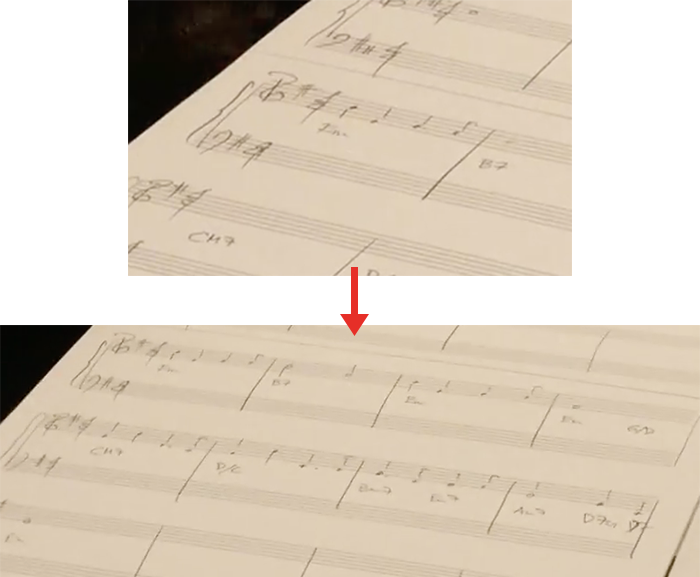
\includegraphics[scale=0.52]{figures/motif-magsalin.png}
		    \caption{A composer continuing his composition with an existing motif. A motif is the main melody that is commonly repeated throughout the composition.}
		    \label{fig:motif-magsalin}
		\end{figure}

		\begin{figure}[H]
			\centering
			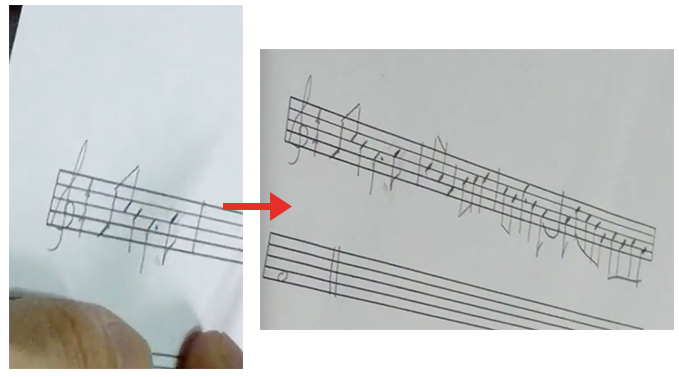
\includegraphics[scale=0.6]{figures/motif-anthony.png}
		    \caption{Another composer demonstrating how he continues his composition with an existing motif.}
		    \label{fig:motif-anthony}
		\end{figure}

		\begin{figure}[H]
			\centering
			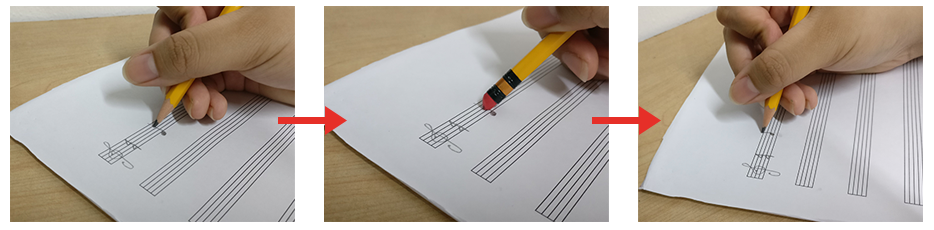
\includegraphics[scale=0.46]{figures/handwritten-transpose-erase.png}
		    \caption{A composer trying to transpose an existing note in the composition. Transposing a note is simply changing its pitch.}
		    \label{fig:handwritten-transpose-erase}
		\end{figure}

		\begin{figure}[H]
			\centering
			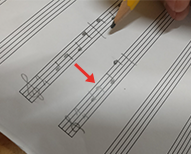
\includegraphics[scale=1.0]{figures/handwritten-transpose-measure.png}
		    \caption{A composer transposing a set of notes to another measure.}
		    \label{fig:handwritten-transpose-measure}
		\end{figure}

		\begin{figure}[H]
			\centering
			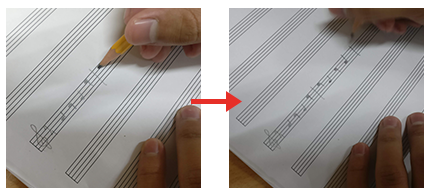
\includegraphics[scale=0.9]{figures/handwritten-retrograde.png}
		    \caption{A composer applying retrograde on a motif. Retrograde is a musical technique where the order of a set of notes are reversed horizontally.}
		    \label{fig:handwritten-retrograde}
		\end{figure}

		From the identified key points, the researchers came up with the affinity diagram shown in Figure \ref{fig:affinity-diagram}. 

		\begin{figure}[H]
			\centering
			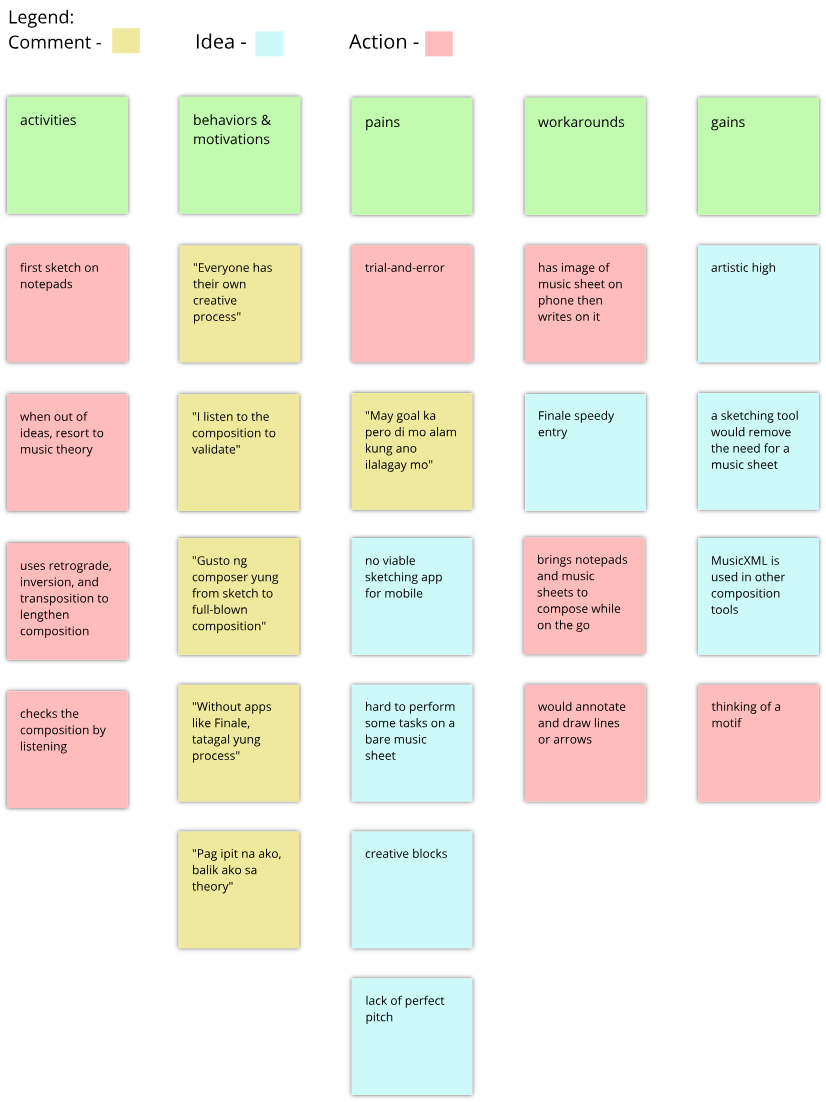
\includegraphics[scale=0.45]{figures/affinity_diagram.png}
		    \caption{The digital version of the affinity diagram taking into account key points from the observations and feedback from the composers. }
		    \label{fig:affinity-diagram}
		\end{figure} 

		\begin{comment}
		>> Observation: "Composers still add notes a few steps above a staff"
		>> Clarification: We asked the composers if these notes mean they are a higher pitch and what are these called?
		>> Verification: We were able to verify that this is called Octava
		>> Translation: We added a feature in the Add Note module where we can add notes a few steps/lines above a staff

		\textbf{Observation:} 	&  \\
	  	\textbf{Clarification:} 	&  \\
	  	\textbf{Verification:} 	&  \\
	  	\textbf{Translation:} 	&  \\
	  	\hline
		\end{comment}

		Table \ref{tab:feature-translations} shows how the identified needs and pain points were translated to features for the developed prototypes.

		\begin{longtable}{|p{2.5cm} p{12.5cm}|}
			\caption{Feature Translations} \label{tab:feature-translations} \\ 
		  	\hline

		  	\textbf{Observation:} 	& Composers would often just write lines as notes and rests on the music sheet. \\
		  	\textbf{Clarification:} 	& Asked the composers why they drew notes and rests like that. \\
		  	\textbf{Verification:} 	& Verified that it felt faster writing them like that. \\
		  	\textbf{Translation:} 	& Added a feature that allowed adding notes and rests on the music sheet. \\
		  	\hline

		  	\textbf{Observation:} 	& Composers would scratch on multiple notes and rests. \\
		  	\textbf{Clarification:} 	& Asked the composers why they did that. \\
		  	\textbf{Verification:} 	& Verified that it was faster to remove notes and rests that way than erasing. \\
		  	\textbf{Translation:} 	& Added a feature that allowed deleting multiple notes and rests on the music sheet. \\
		  	\hline

		  	\textbf{Observation:} 	& Composers would erase old notes/rests and write new notes/rests on top. \\
		  	\textbf{Clarification:} 	& Asked the composers if that was how they would always edit notes/rests. \\
		  	\textbf{Verification:} 	& Verified that they always did that even though it was tedious. \\
		  	\textbf{Translation:} 	& Added a feature that allowed editing notes/rests in the music sheet. \\
		  	\hline

		  	\textbf{Observation:} 	& Composers would start compositions by writing the time signature. \\
		  	\textbf{Clarification:} 	& Asked if they always started with the time signature. \\
		  	\textbf{Verification:} 	& Verified that they would often decide on the time signature as well as the key signature at the start and would rarely change it. \\
		  	\textbf{Translation:} 	& Added a feature that allowed changing the time and key signature. \\
		  	\hline

		  	\textbf{Observation:} 	& Composers played some of their compositions that seemed to repeat a certain melody. \\
		  	\textbf{Clarification:} 	& Asked why it was like that and how they did that. \\
		  	\textbf{Verification:} 	& Verified that they would sometimes compose whole compositions using just one melody or motif that was modified repeatedly using transposition, or retrograde/inversion. \\
		  	\textbf{Translation:} 	& Added a feature that allowed transposition and retrograde/inversion. \\
		  	\hline

		  	\textbf{Observation:} 	& Composers wrote annotations or drew arrows on the music sheet that pointed to a specific set of notes/rests. \\
		  	\textbf{Clarification:} 	& Asked why they did that and what it was for. \\
		  	\textbf{Verification:} 	& Verified that they did that to denote repeating or ``copying'' the set of notes since it was faster than rewriting them. \\
		  	\textbf{Translation:} 	& Added a feature that allowed cut, copy, or paste. \\
		  	\hline

		  	\textbf{Observation:} 	& Composers would use the piano or a guitar repeatedly while writing on a music sheet. \\
		  	\textbf{Clarification:} 	& Asked why they did that. \\
		  	\textbf{Verification:} 	& Verified that they did that since they did not have ``perfect pitch'' and could not test the pitch without actually hearing it. \\
		  	\textbf{Translation:} 	& Added a music playback feature for playing the whole composition and when adding notes.  \\
		  	\hline

		  	\textbf{Observation:} 	& Composers would draw sharps on flats in the middle of their composition. \\
		  	\textbf{Clarification:} 	& Asked what those were for and why they had to do that. \\
		  	\textbf{Verification:} 	& Verified that they did that to modify the pitch quickly without having to change the whole key signature. \\
		  	\textbf{Translation:} 	& Added a feature that allowed adding and removing accidentals.  \\
		  	\hline

		  	\textbf{Observation:} 	& Composers sometimes write an ``8va'' on top of notes. \\
		  	\textbf{Clarification:} 	& Asked the composers what these do and what are they called. \\
		  	\textbf{Verification:} 	& Verified that it was called ottava and they raise the pitch of the note to the next octave. \\
		  	\textbf{Translation:} 	& Added a feature that allowed placing ottava and its counterpart, ottava bassa on notes. \\
		  	\hline
		\end{longtable}

	\section{Design and Implementation of Interaction}
	\label{sec:design}

		\subsection{Initial Sketches}

			\begin{figure}[H]
				\centering
				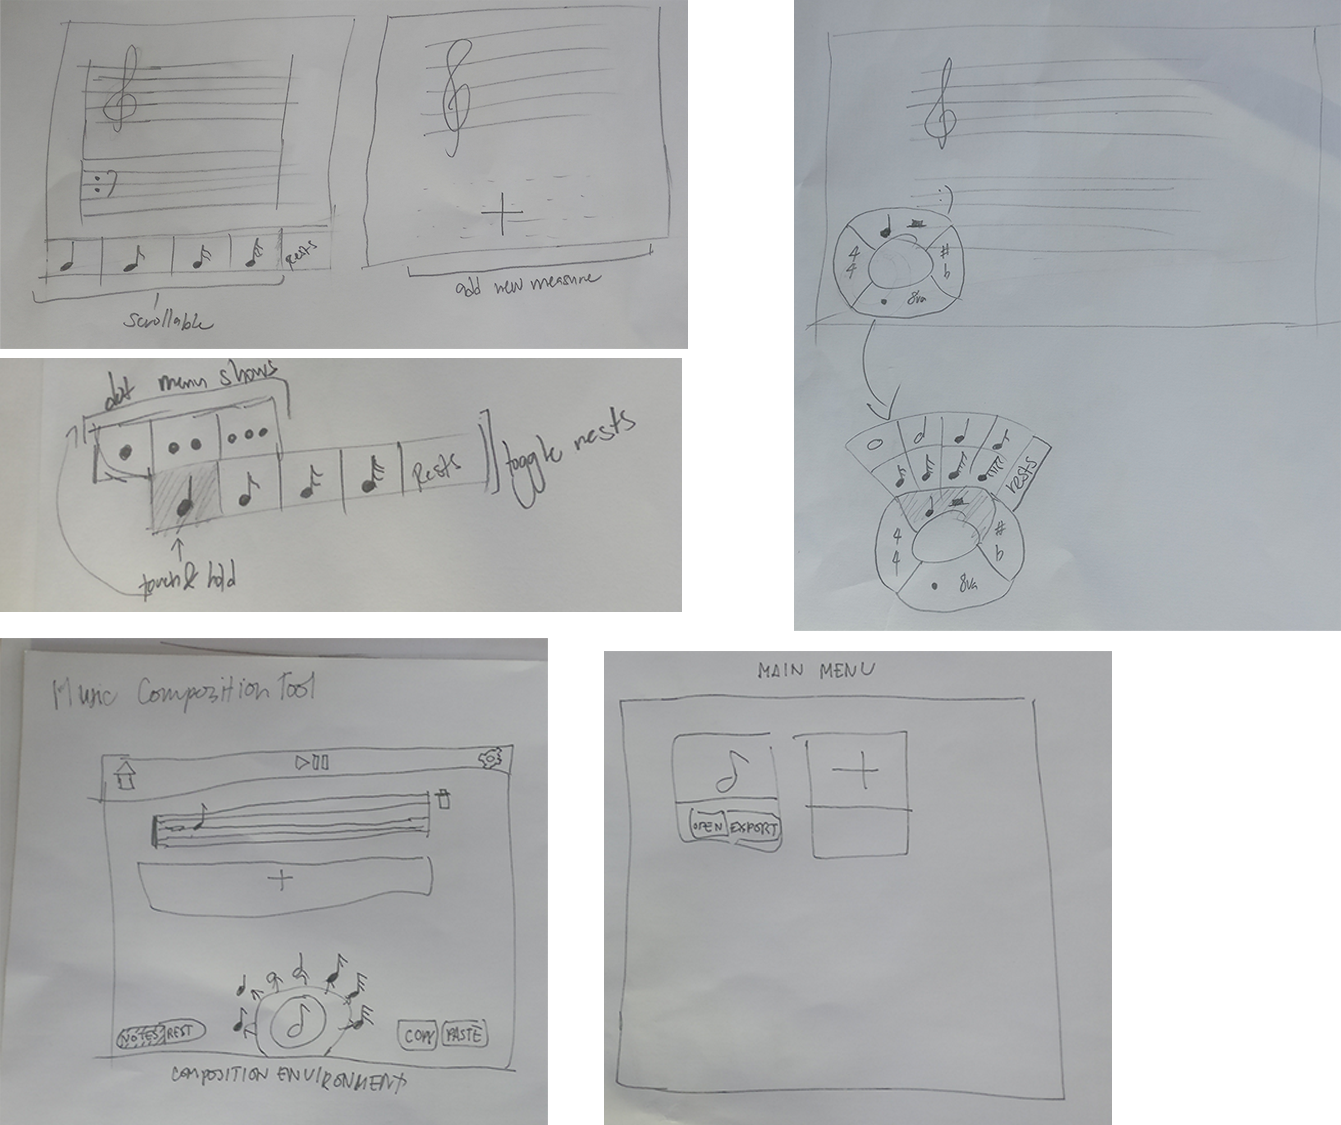
\includegraphics[scale=0.3]{figures/initial_sketches.png}
			    \caption{Sketches of the initial user interface and interaction design.}
			    \label{fig:initial_sketches}
			\end{figure}

			%The initial sketches (see Figure \ref{fig:initial_sketches}) were made to quickly ideate possible designs and interactions for the system. The researchers made several of these to see how different interactions would work. However, given the limited medium, only the core features (adding, editing, and deleting) were focused on. Most of the differences from the sketches involved the add function. In the first sketch (see Figure \ref{fig:initial_sketches} S1), adding was done by dragging a desired note/rest from the radial menu to the measure. The second sketch (see Figure \ref{fig:initial_sketches} S2) on the other hand, did adding through a radial menu which was accessed by holding on any part of the measure and dragging the finger or tapping on the desired item. The last sketch (see Figure \ref{fig:initial_sketches} S3) was a bit similar to the first one since it was also drag-and-drop interaction, but instead used a scrollable menu. 

			The initial sketches (see Figure \ref{fig:initial_sketches}) were made to quickly ideate possible designs and interactions for the system. The researchers made several of these to see how different interactions would work. However, given the limited medium, only the core features (adding, editing, and deleting) were focused on. The researchers then picked the interactions and designs from the sketches that felt easiest to perform.

		\subsection{Mid-fidelity Prototypes}
		\label{sec:mid-fidelity-prototypes}

			\begin{figure}[H]
				\centering
				\frame{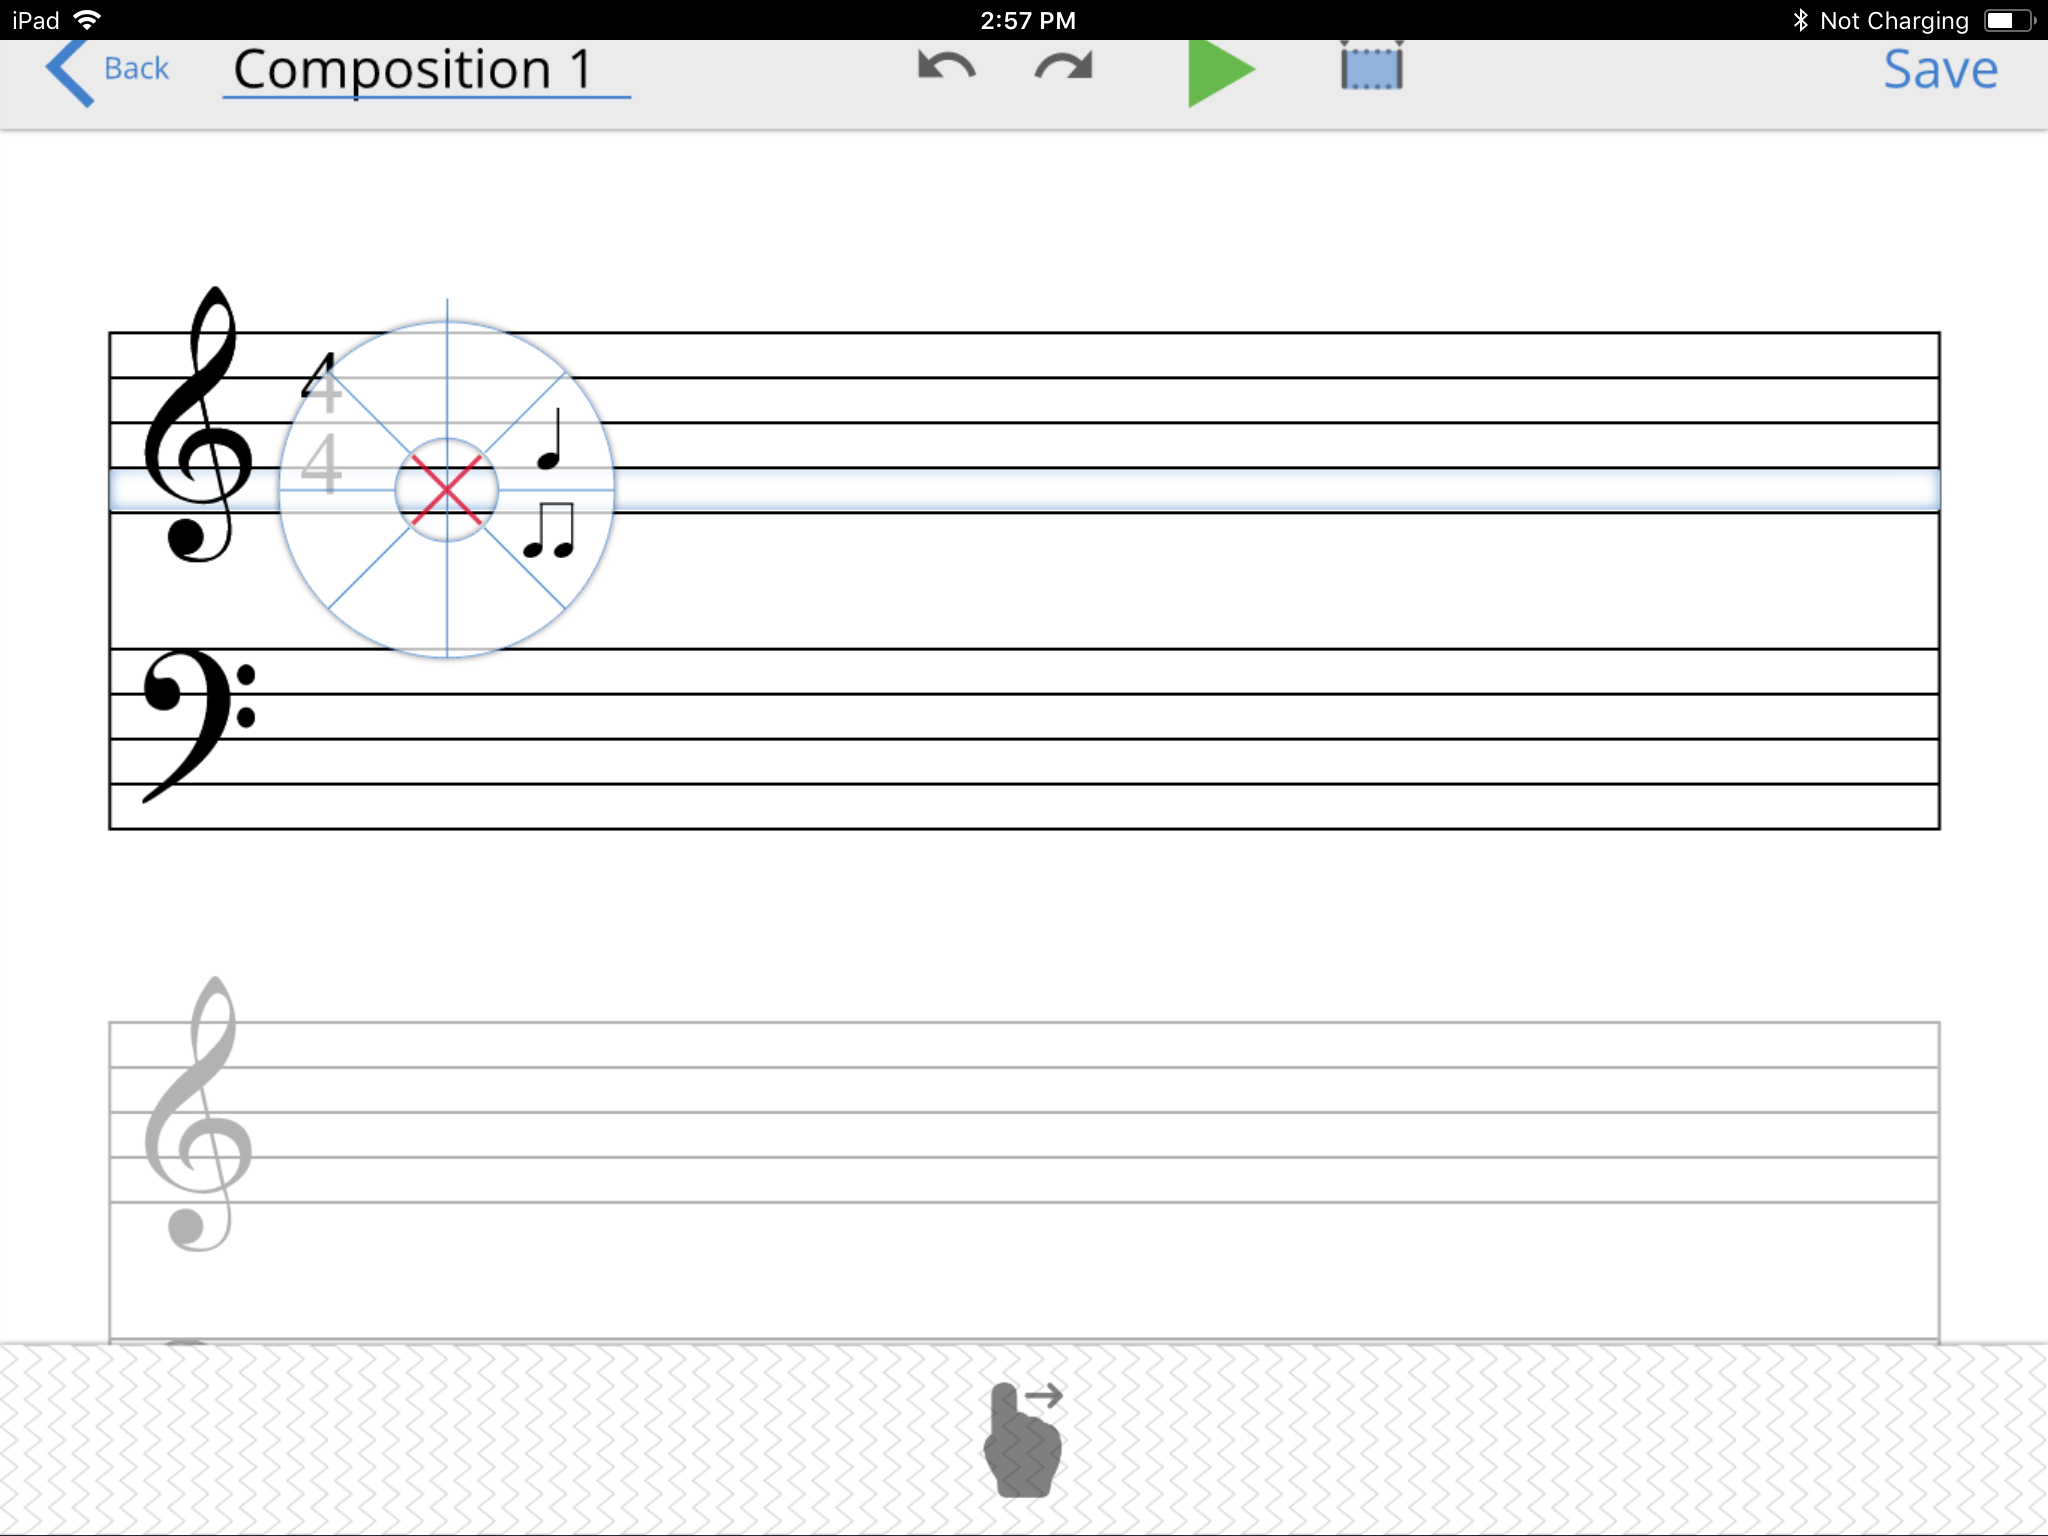
\includegraphics[scale=0.15]{figures/invision_v1}}
			    \caption{The first version of the mid-fidelity prototype built using InVision.}
			    \label{fig:invision_v1}
			\end{figure} 

			The consolidated design from the sketches resulted in the mid-fidelity prototype shown in Figure \ref{fig:invision_v1}. Since adding and editing was one of the tasks that composers would be doing the most, they needed to be the easiest to perform. The add and edit feature took inspiration from the study by \citet{zhao2007earpod} which used a circular menu to make selecting items easier through muscle memory. The idea was to create a similar interaction so that through repetitive use, adding and editing would be done through muscle memory removing the need to consciously think about the actual interaction. The notes and rests menu showed by holding on a line or space on the measure. Users can then select a note or rests by either dragging their finger to the button of the note or rest and lifting it, or by simply tapping on it. 

			A gesture space was also added at the bottom part of the screen for more advanced tasks like highlighting, transposition, retrograde, inversion, and musical metacreation. Users only needed to perform or ``draw'' certain swipe gestures on the space to use the said features, making it follow how they would usually ``draw'' on a music sheet. 

			\begin{figure}[H]
				\centering
				\frame{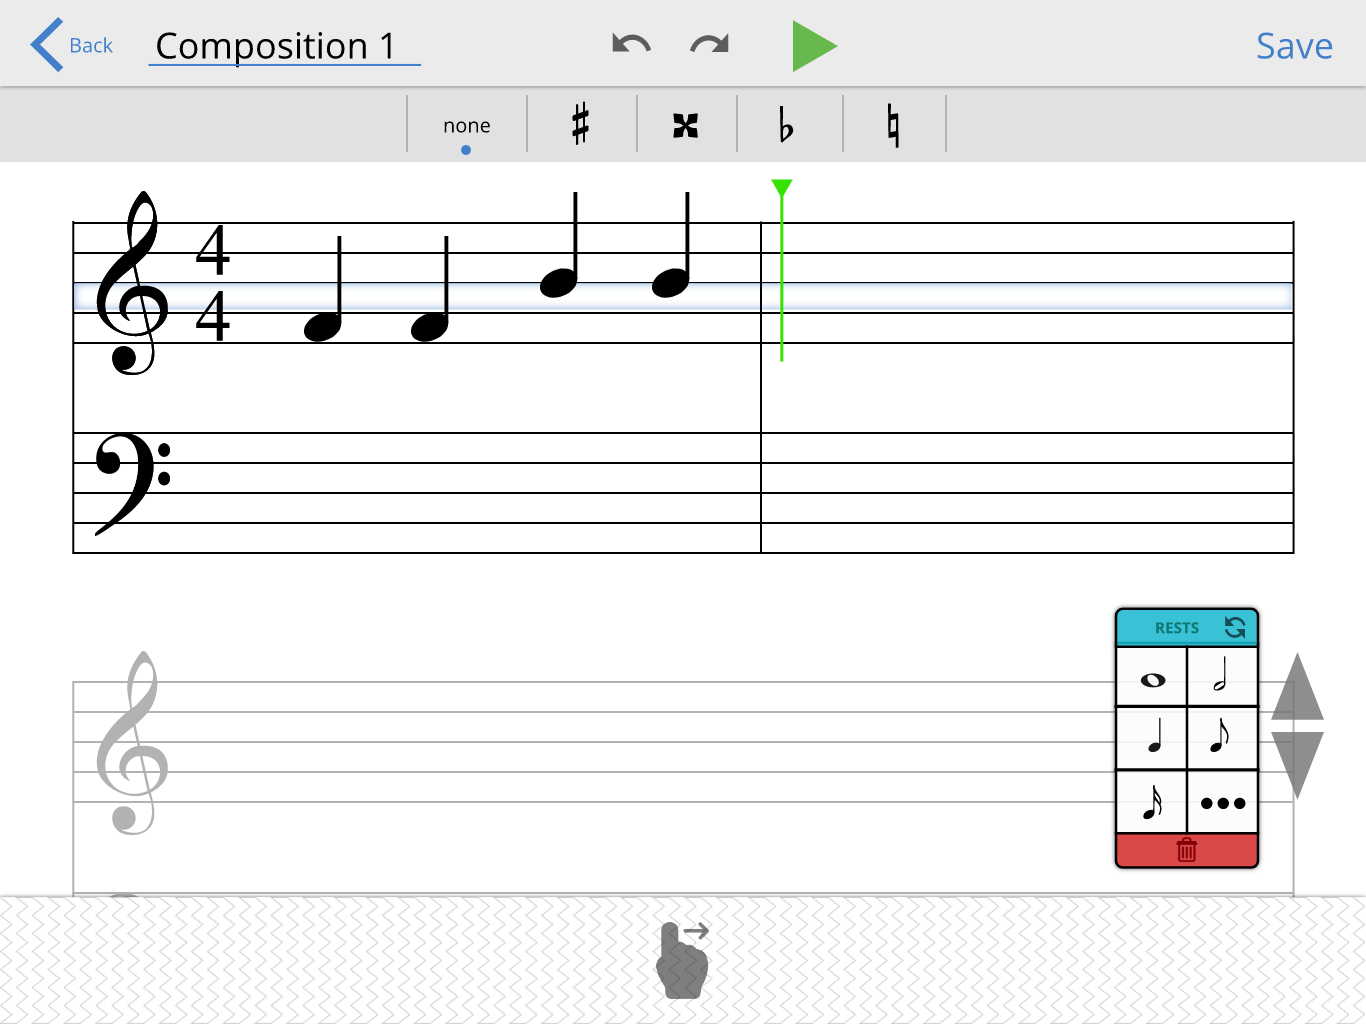
\includegraphics[scale=0.2]{figures/invision_v2}}
			    \caption{The second version of the mid-fidelity prototype built using InVision.}
			    \label{fig:invision_v2}
			\end{figure} 

			The second version of the mid-fidelity prototype changed the method of adding and editing. It was found that the hold interaction was a bit slow, especially since it was essential for a lot of composers that they could quickly add notes or rests when they had an idea in mind. The revised interaction added the cursor and arrow keys as well as the always present notation menu. Users can then add and edit notes using the notation menu with the selected notes or rests appearing in the location of the cursor. This new interaction was found to be simpler and faster, requiring less time and effort from the composers to perform. Although the interface changed a bit across the iterations, this method of interaction was used until the last version of the application. 

		\subsection{High-fidelity Prototypes}
		\label{sec:high-fidelity-prototypes}

			\subsubsection{Iteration 1}

				\begin{figure}[H]
					\centering
					\frame{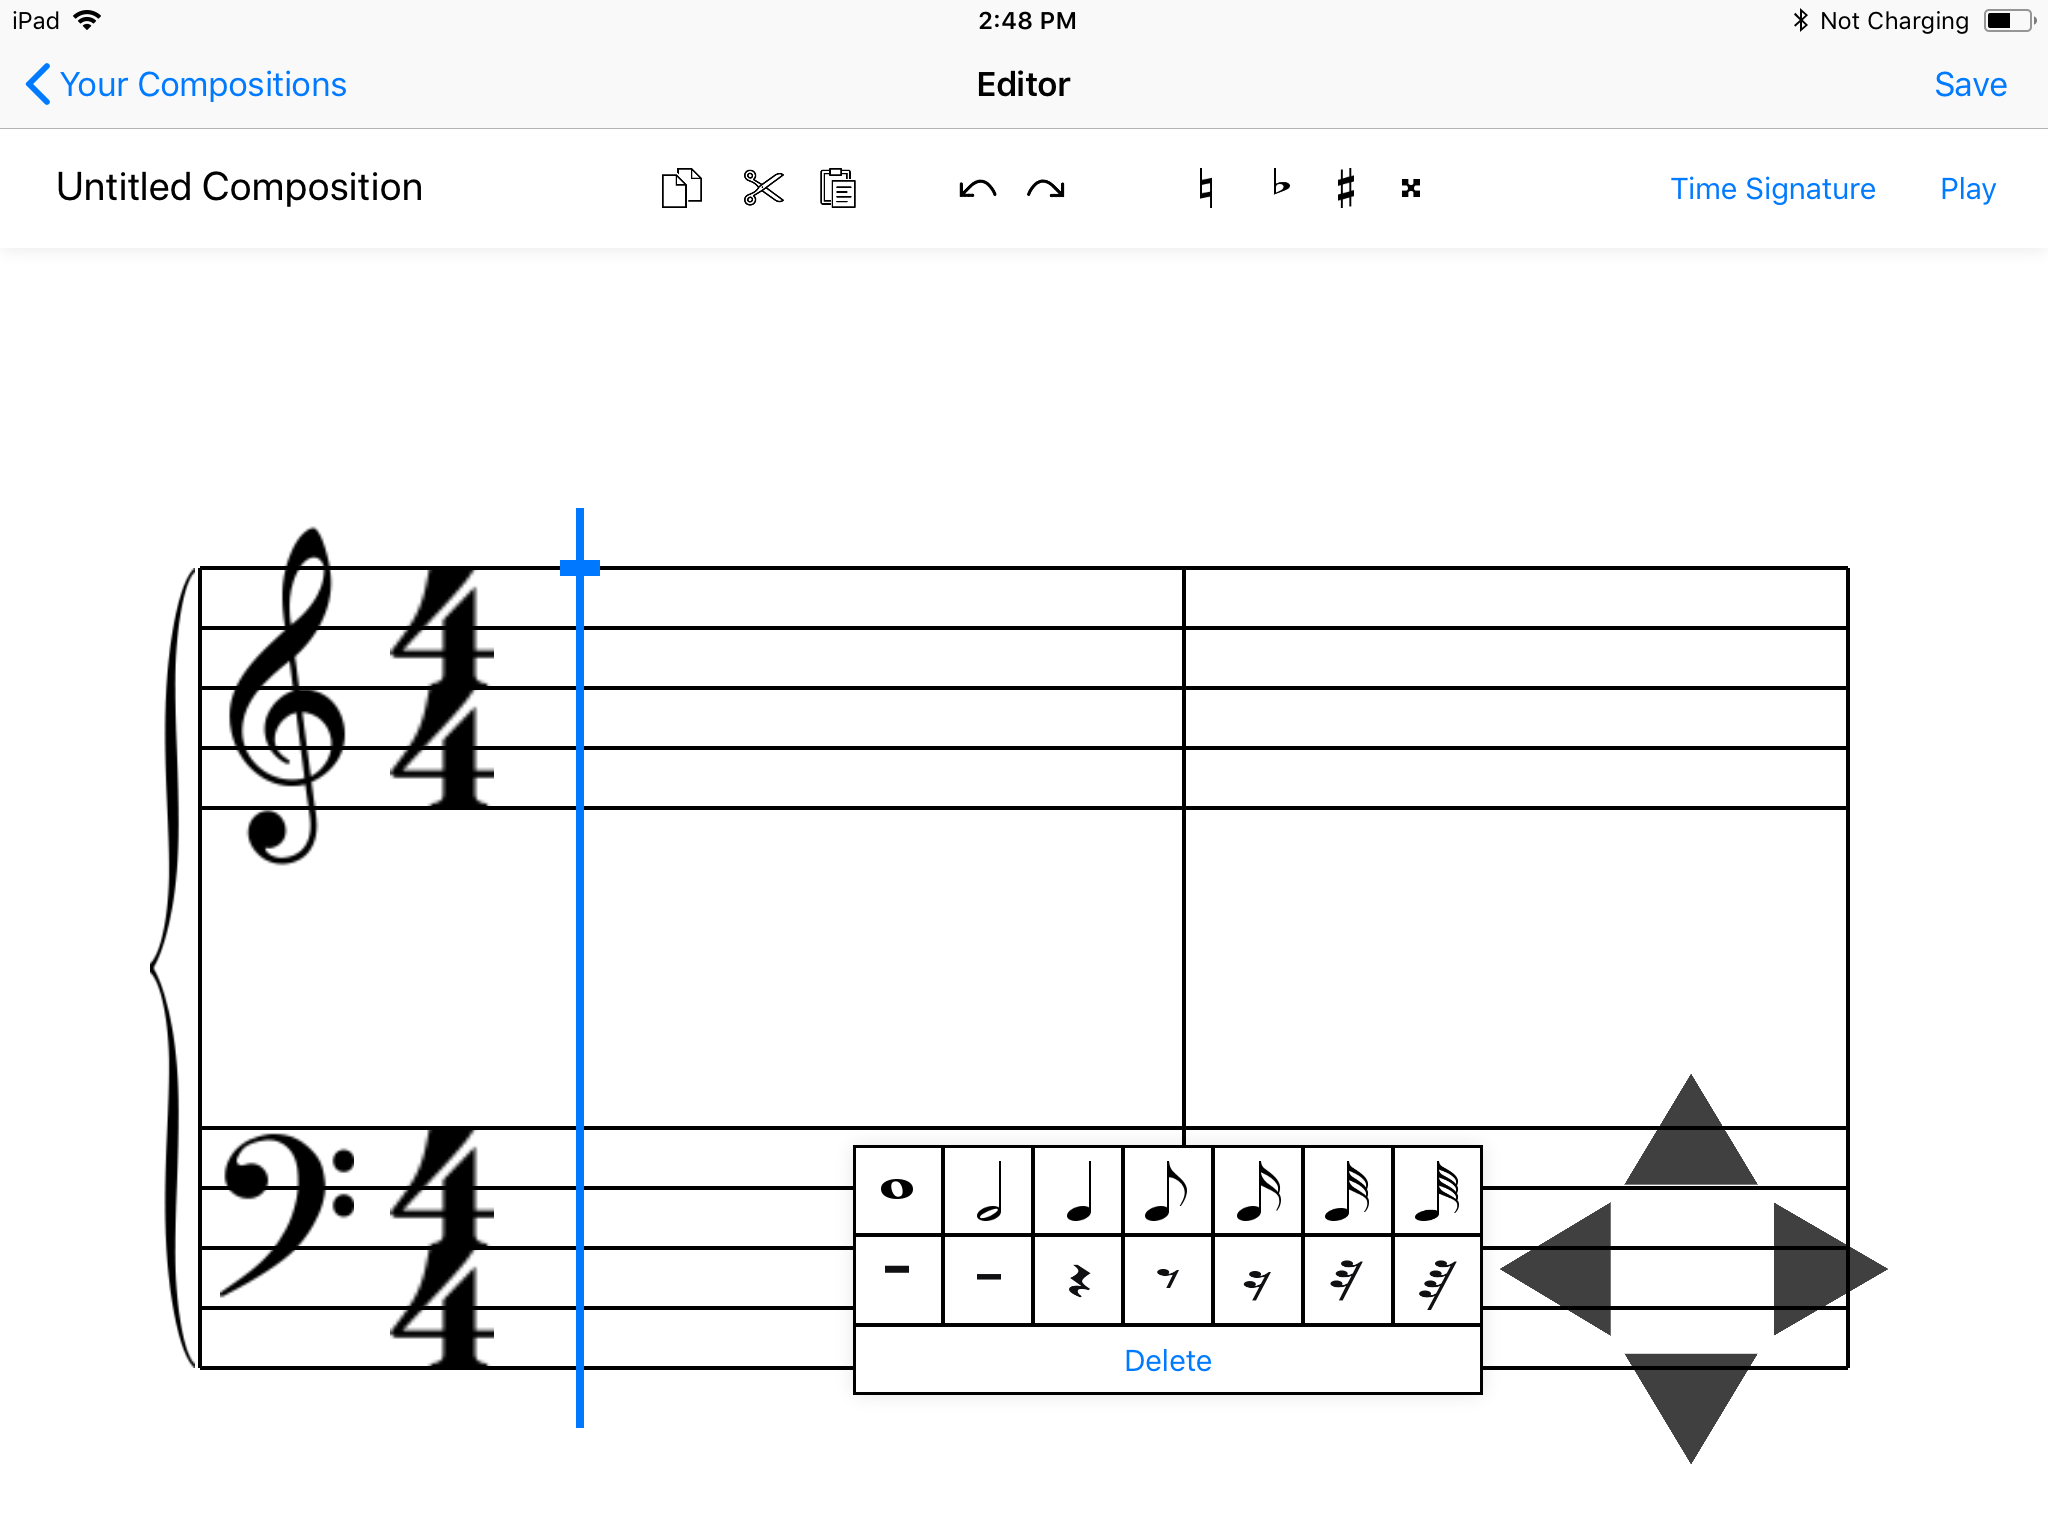
\includegraphics[scale=0.15]{figures/flow_it1.PNG}}
				    \caption{The first version of the high-fidelity prototype built using Swift.}
				    \label{fig:flow_it1}
				\end{figure} 


				The first version of the high-fidelity prototype (see Figure \ref{fig:flow_it1}) was still a bit similar to the second version of the mid-fidelity prototype (see Figure \ref{fig:invision_v2}). However, the gesture space was removed and was planned to be replaced with specific gestures and buttons to save screen space. The highlight was delegated to a two-finger drag gesture so it would not conflict with the one-finger drag gesture for scroll. A full set of arrow keys was added to control the cursor, taking inspiration from the ``speedy entry'' from Finale where users would press the arrow keys on the keyboard to move the cursor that tells where the note or rest would appear. However, users were also given the ability to tap on any valid location they wanted on the measure to move the cursor. 

			\subsubsection{Iteration 2}

				\begin{figure}[H]
					\centering
					\frame{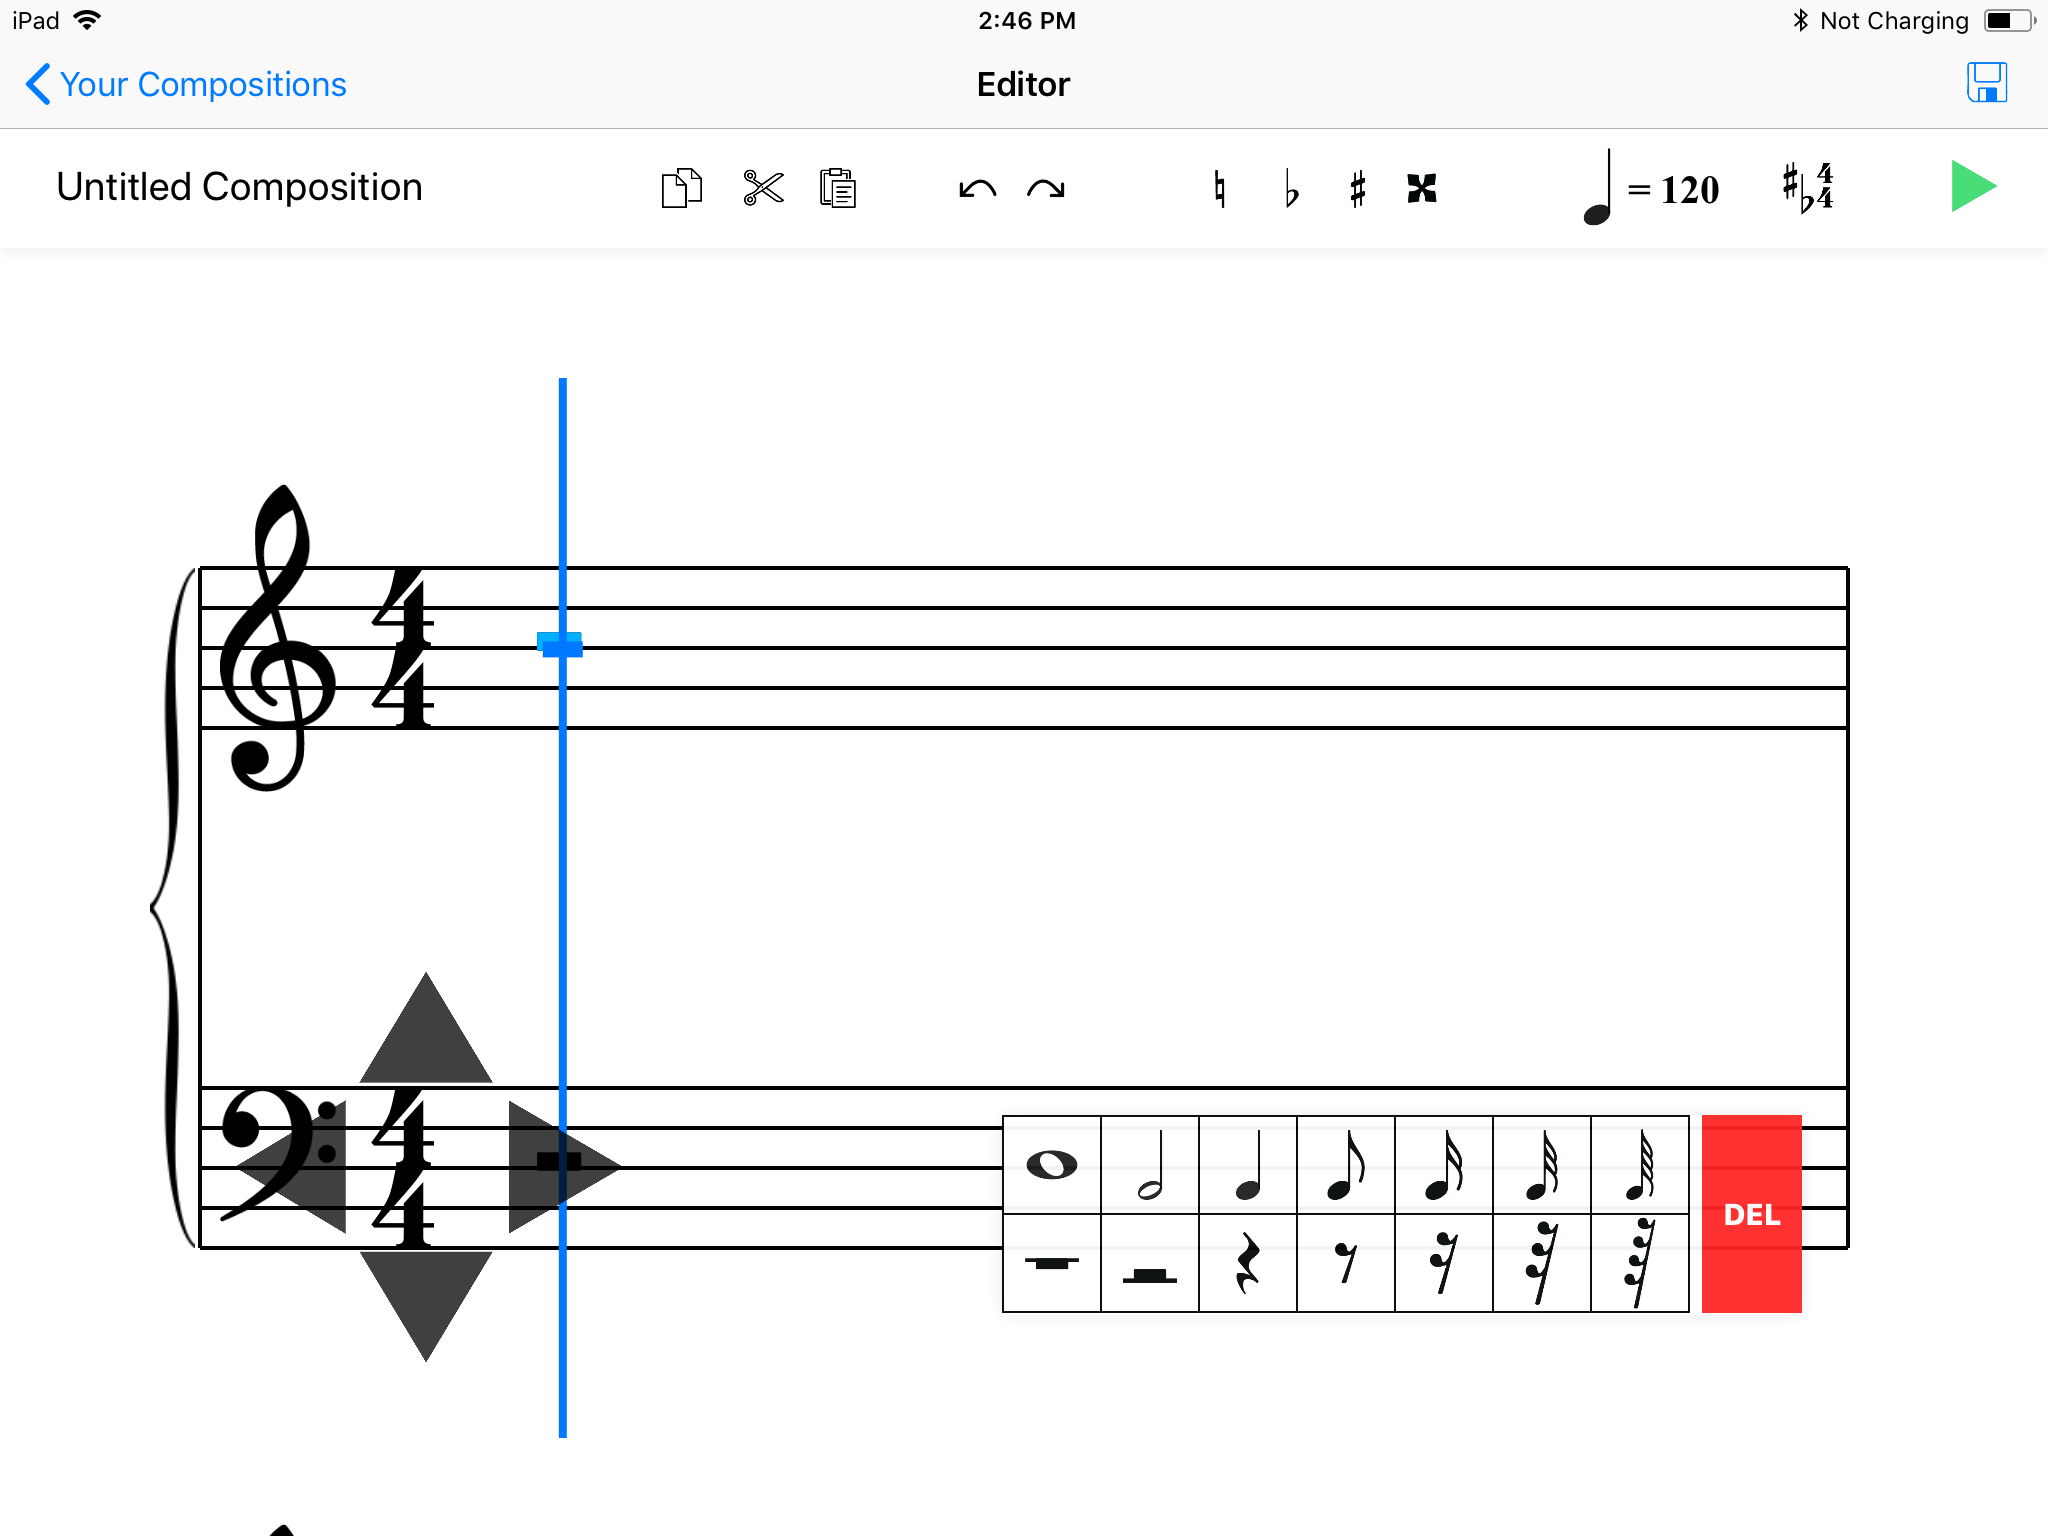
\includegraphics[scale=0.15]{figures/flow_it2.PNG}}
				    \caption{The second version of the high-fidelity prototype built using Swift.}
				    \label{fig:flow_it2}
				\end{figure} 

				The biggest change for iteration 2 came with the revised highlight interaction. From the user tests, it was found that the two-finger drag for highlight in the previous iteration was hard to figure out. This was evident from the quantitative data gathered which showed the \textit{Highlight/Select a Group of Notes} having a score of only 2.5 (see Table \ref{tab:results-features-it1} item 6). This also affected the scores of the \textit{Edit a Highlighted/Selected Group of Notes} and \textit{Delete a Highlighted/Selected Group of Notes} features, giving them both one of the lowest scores of 2.2 (see Table \ref{tab:results-features-it1} items 7 and 8 respectively). It was observed that they would try to use a one-finger drag to highlight (see Figure \ref{fig:video_highlight}). Hence, the gestures for the highlight and scroll interactions were switched, resulting in the highlight using only a one-finger drag, while the scroll used a two-finger drag (see Figure \ref{fig:highlight}). 

				\begin{figure}[h]
					\centering
					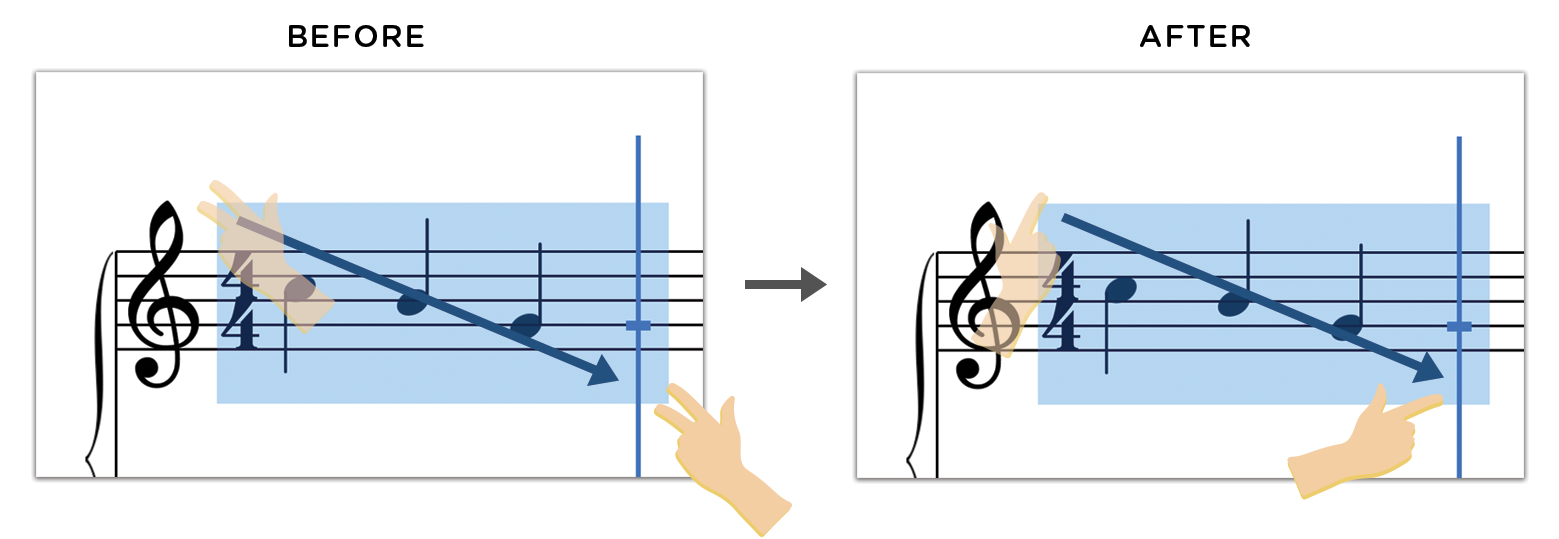
\includegraphics[scale=0.25]{figures/before-after-highlight.png}
				    \caption{The highlight interaction before and after changes were made due to the user testing. The new interaction uses only one (1) finger.}
				    \label{fig:highlight}
				\end{figure}

				Other major changes for iteration 2 were with the menus. In iteration 1, the arrow keys and the notation menu were tied to each other. This meant that if the user moved the arrow keys, the notation menu would follow. However, the researchers soon realized from the user tests that not everyone held the iPad the same way. Some held it with both hands like they would hold a video game controller, making the setup of the two menus a bit unnatural for them. For the second version, the two menus were separated from each other making it possible to rearrange them. 

				%Place image of anthony here

				\begin{figure}[h]
					\centering
					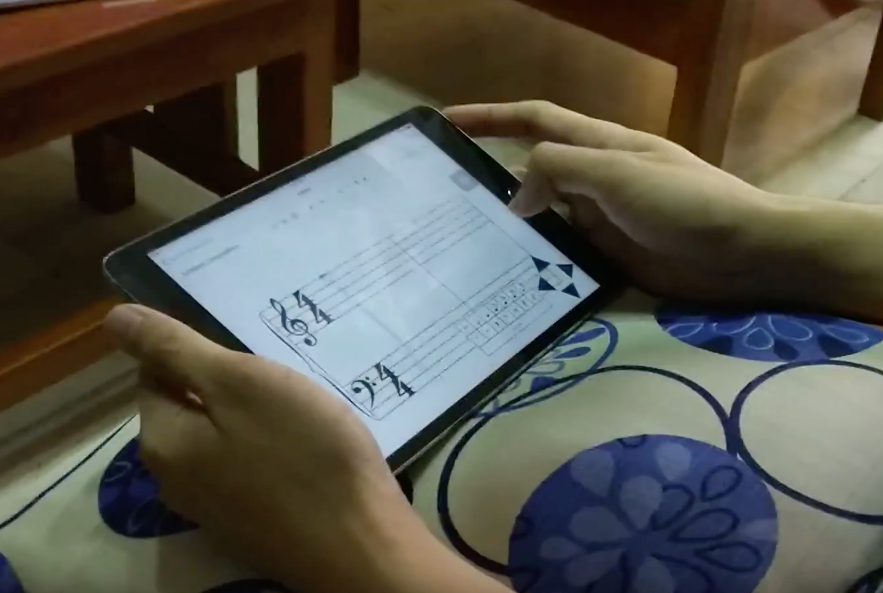
\includegraphics[scale=0.3]{figures/anthony-handheld-ipad.png}
				    \caption{A tester holding the iPad like a video game controller.}
				    \label{fig:handheld_ipad}
				\end{figure}

				The delete button was also moved from the bottom of the notation menu to its side and changed to the color red. The change made the button easier to press and more obvious. 

			\subsubsection{Iteration 3}

				\begin{figure}[H]
					\centering
					\frame{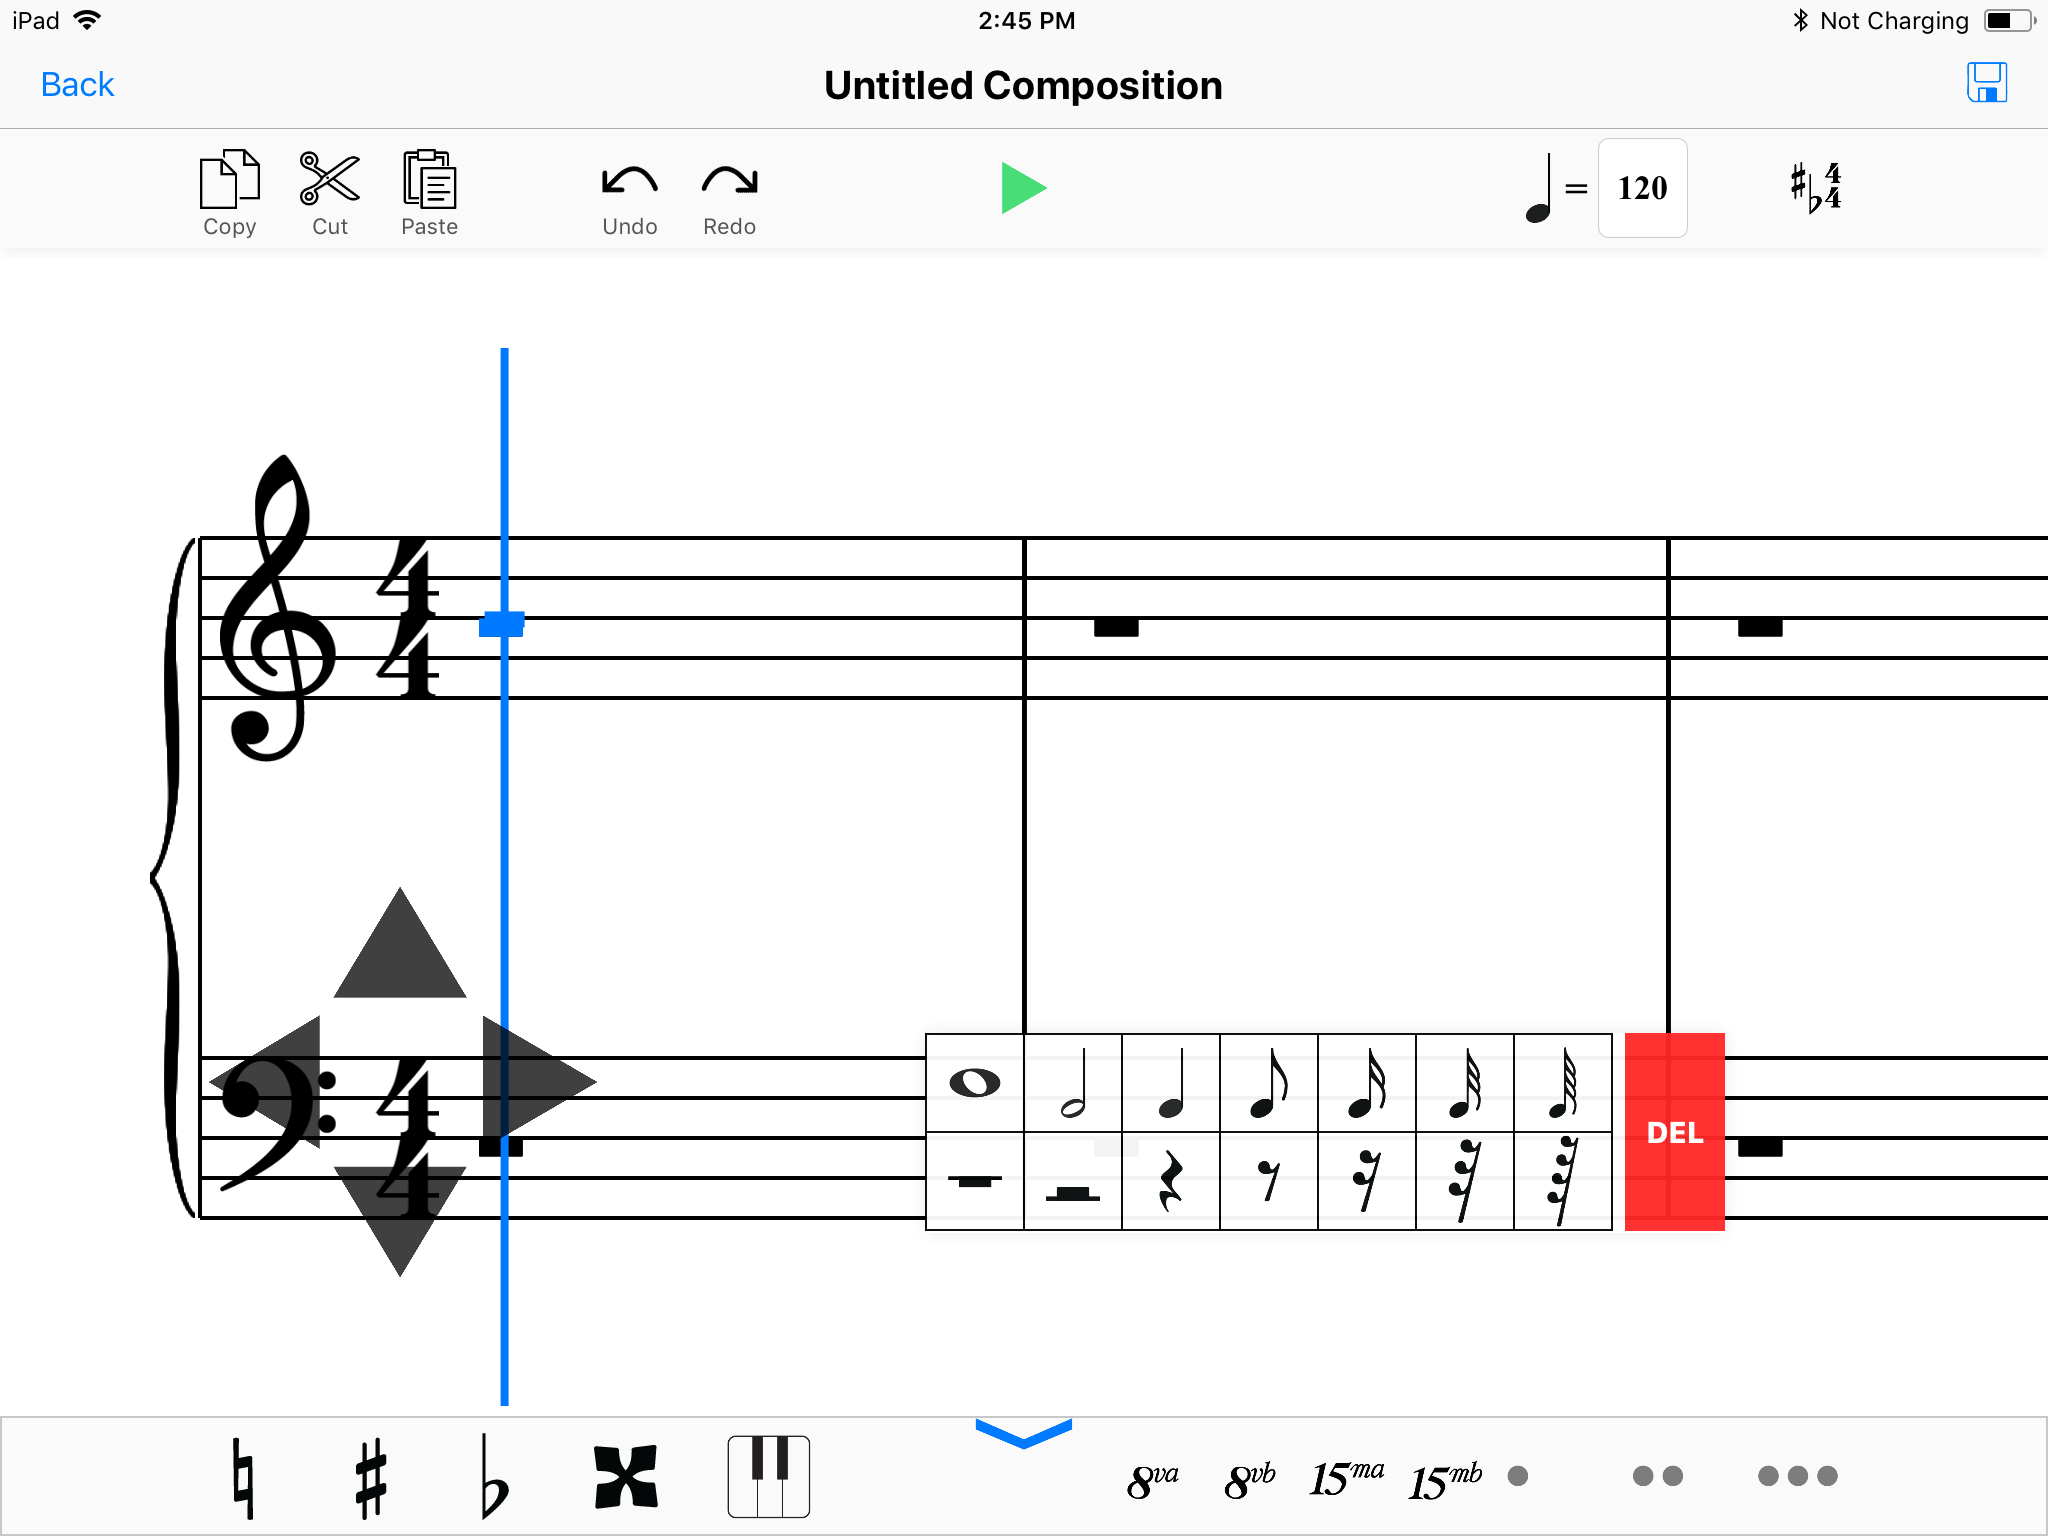
\includegraphics[scale=0.15]{figures/flow_it3.PNG}}
				    \caption{The third version of the high-fidelity prototype built using Swift.}
				    \label{fig:flow_it3}
				\end{figure} 

				Iteration 3 added a new bottom menu containing modifiers like accidentals, dots, and ottavas. This was done so that the top menu would not be crowded. A keyboard, which can be shown using the show/hide keyboard button, was also added to allow users to test out melodies on the keyboard while composing. 

				This version improved on the time and key signature menu (see Figure \ref{fig:before-after-tsmenu}). In the previous version, users had a hard time with the menu because of the sliders. For the quantitative feedback, the \textit{Change Time Signature} feature received a score of 3.2 while the \textit{Change Key Signature} scored a 3.5 (see Table \ref{tab:results-features-it2} items 10 and 11 respectively). Although they were not very low, the qualitative data shows that the sliders made selecting inaccurate and tedious (see Figures \ref{fig:video_timesig} and \ref{fig:video_keysig}). For iteration 3, buttons for common time signatures were added, but users could also type the time signatures they wanted using the keyboard. The key signature menu was redesigned to be a circular menu that follows the circle of fifths. 

				\begin{figure}[H]
					\centering
					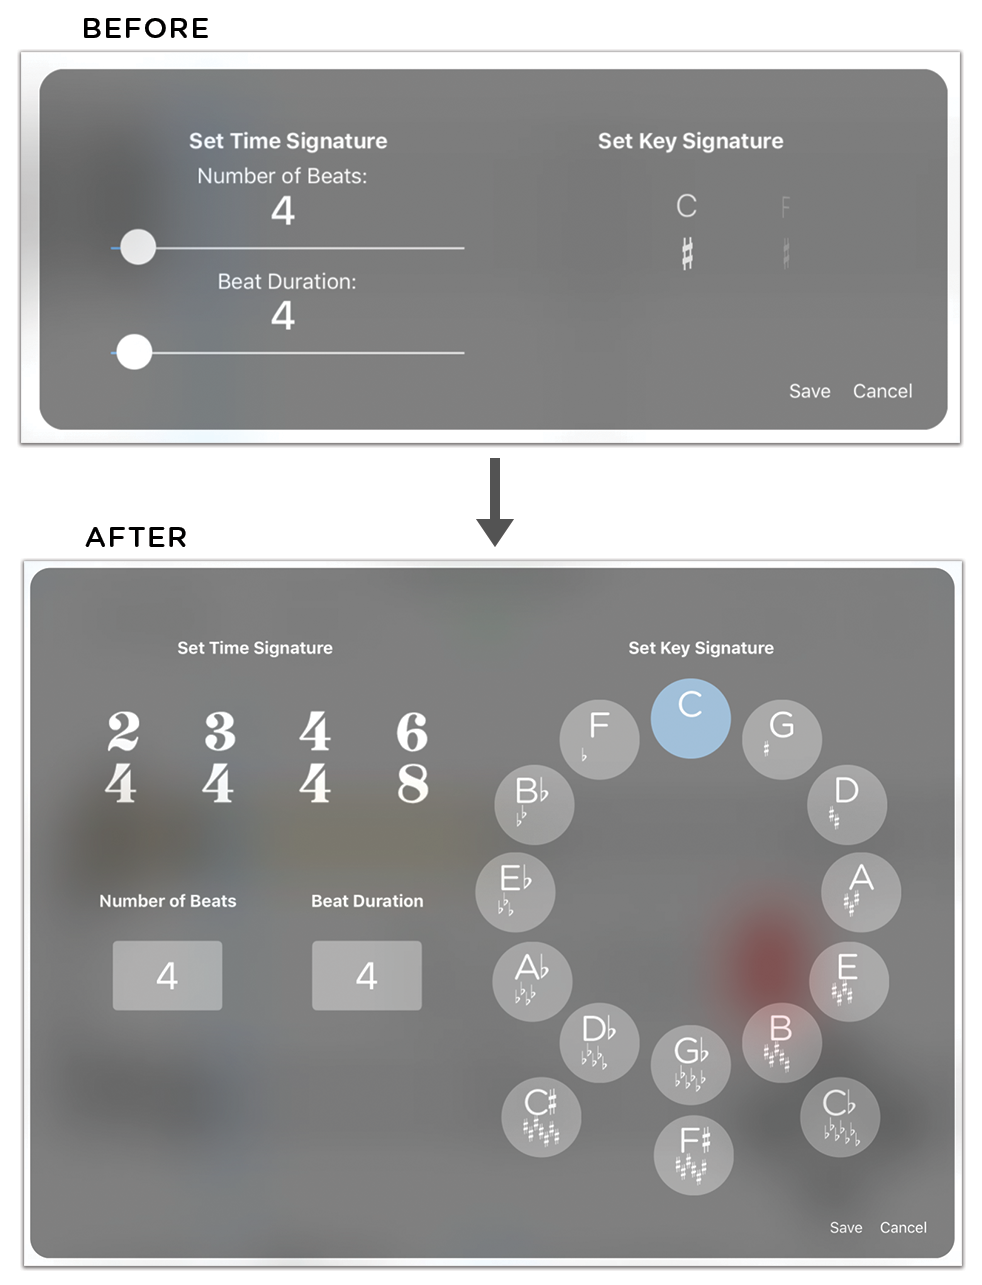
\includegraphics[scale=0.34]{figures/before-after-tsmenu}
				    \caption{The time and key signature menu before and after changes were made due to the user testing. Sliders in the previous iteration made selecting inaccurate and tedious (see Figures \ref{fig:video_timesig} and \ref{fig:video_keysig}). The revised time signature menu adds buttons for the common time signatures and also allows users to input any valid time signature they want. The revised key signature menu is now circular and follows the circle of fifths.}
				    \label{fig:before-after-tsmenu}
				\end{figure} 

				The transpose interaction was also revised, giving it a totally new menu that shows when a group of notes are highlighted (see Figure \ref{fig:before-after-transpose}). This was done to make the transpose interaction more obvious to the users.

				% TRANSPOSE VIDEO REFERENCE

				\begin{figure}[h]
					\centering
					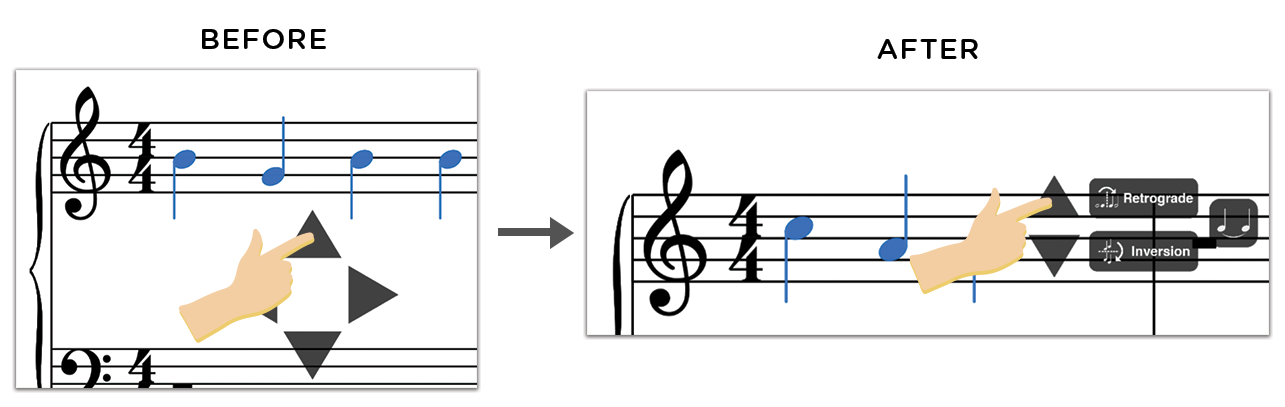
\includegraphics[scale=0.32]{figures/before-after-transpose}
				    \caption{The transpose interaction before and after changes were made due to the user testing. The new transpose interaction adds a menu containing separate transpose arrow keys as well as additional modifiers.}
				    \label{fig:before-after-transpose}
				\end{figure}

			\subsubsection{Iteration 4}

				\begin{figure}[H]
					\centering
					\frame{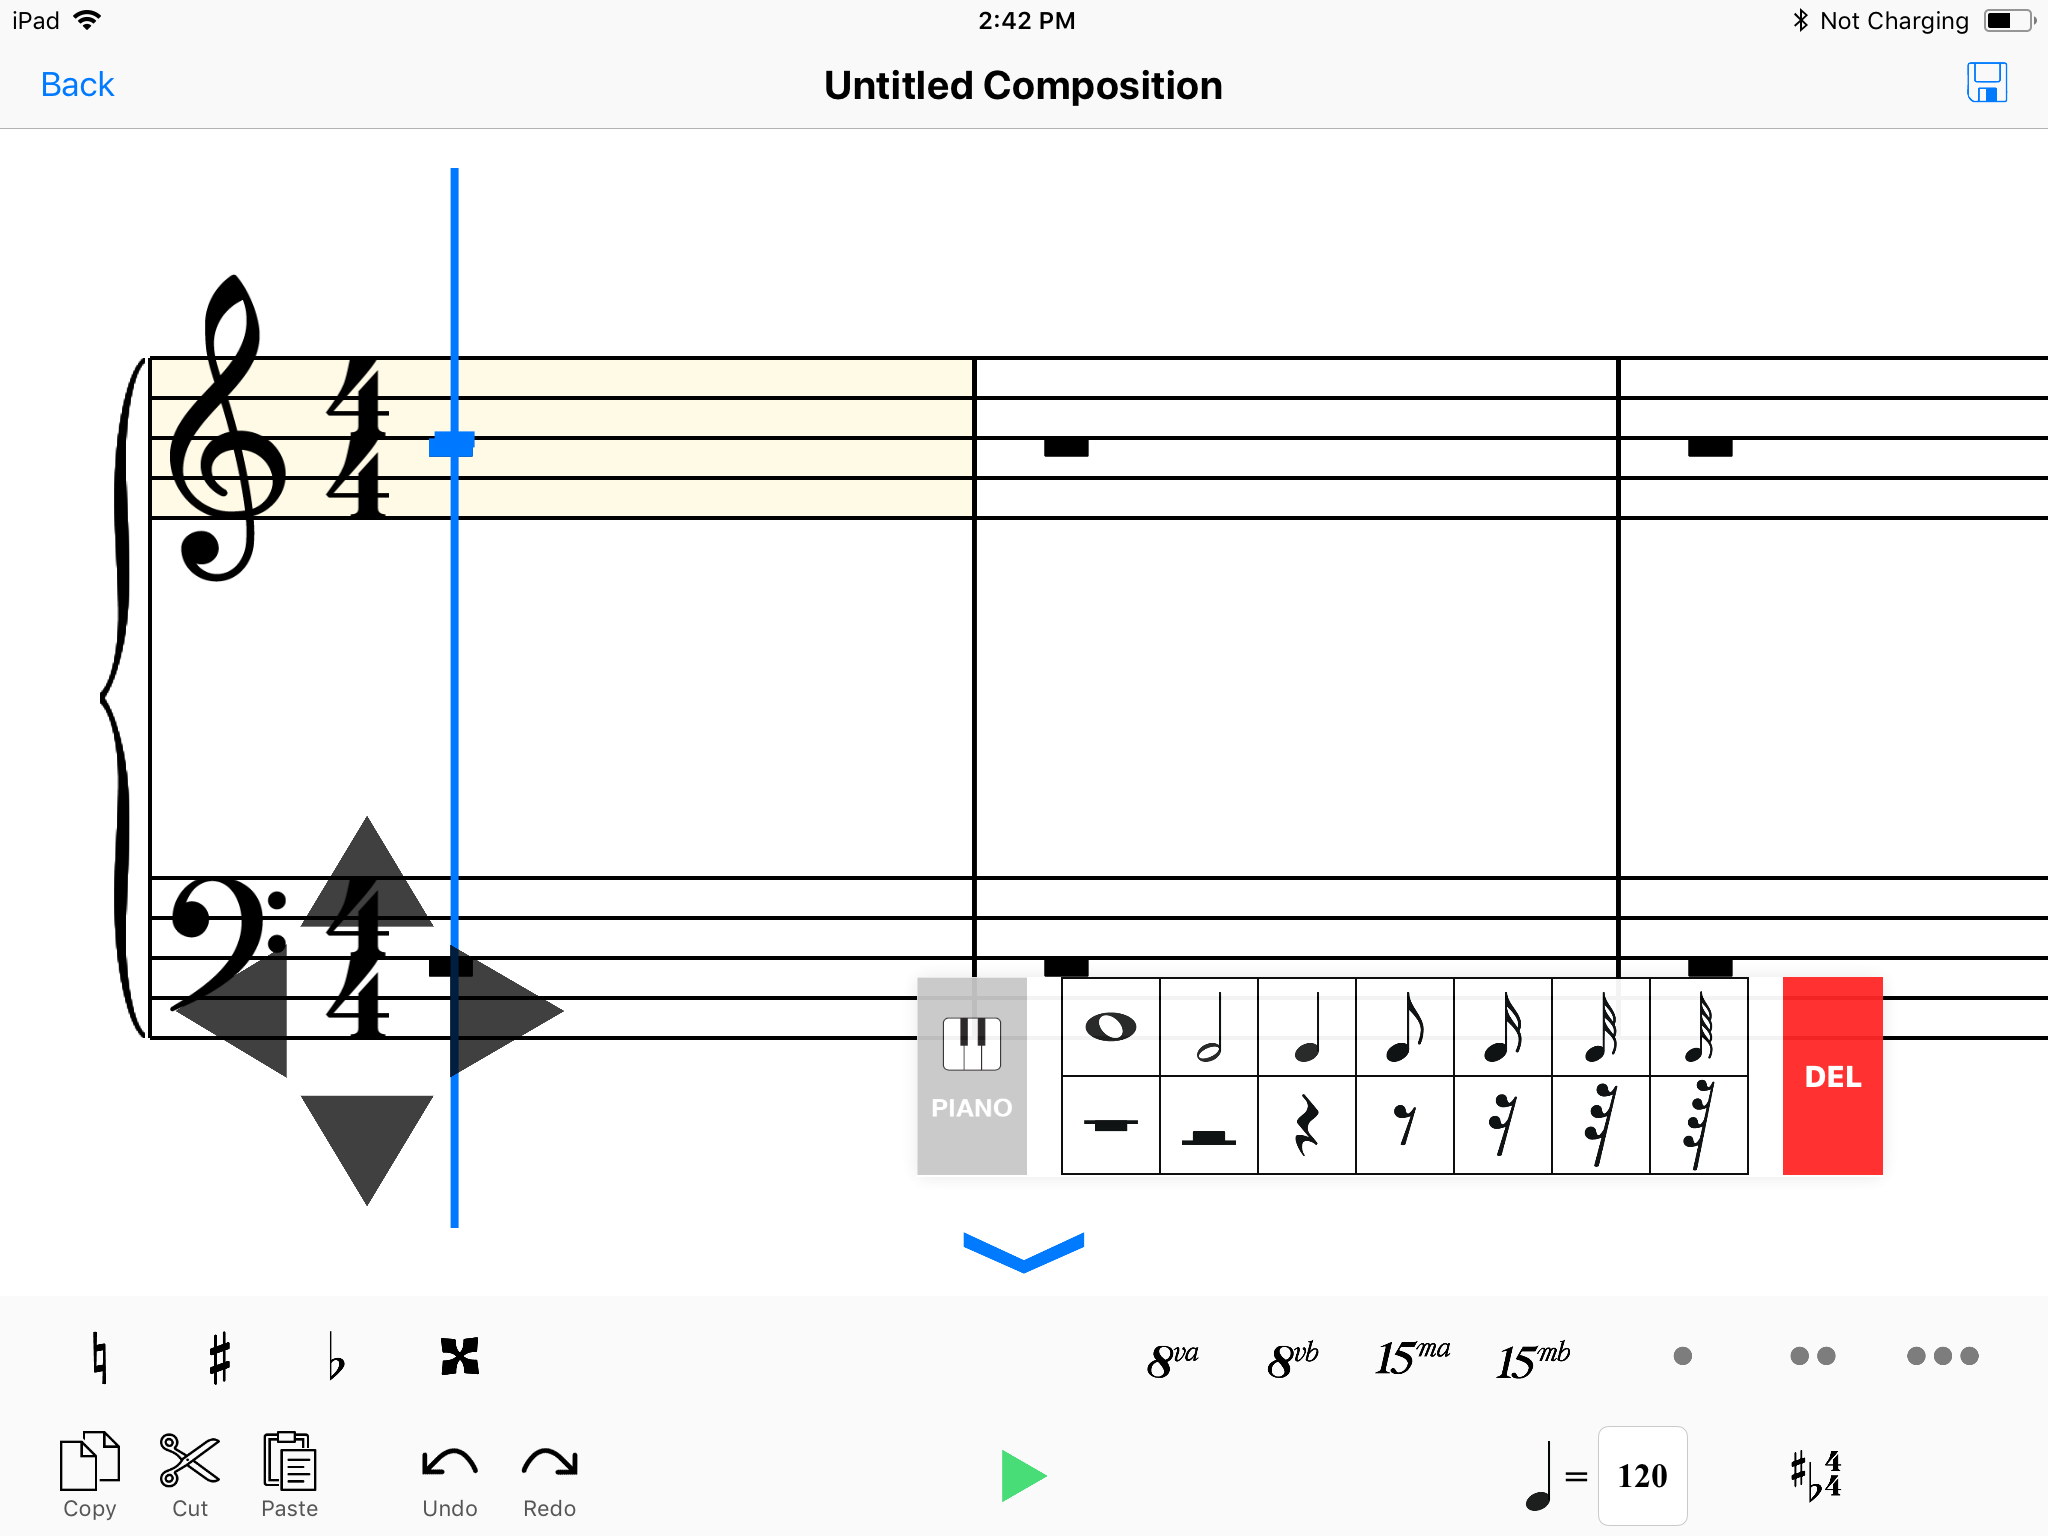
\includegraphics[scale=0.15]{figures/flow_it4.PNG}}
				    \caption{The fourth version of the high-fidelity prototype built using Swift.}
				    \label{fig:flow_it4}
				\end{figure} 

				It was observed from the tests that having two menus on opposite sides of the screen split the focus of the users. They would first try to search for features at the bottom menu and would sometimes forget that there was also a menu at the top (see Figure \ref{fig:video_menu}). So for iteration 4, the top menu was moved to the bottom allowing users to focus on only one part of the screen when looking for features (see Figure \ref{fig:before-after-menu}). 

				\begin{figure}[h]
					\centering
					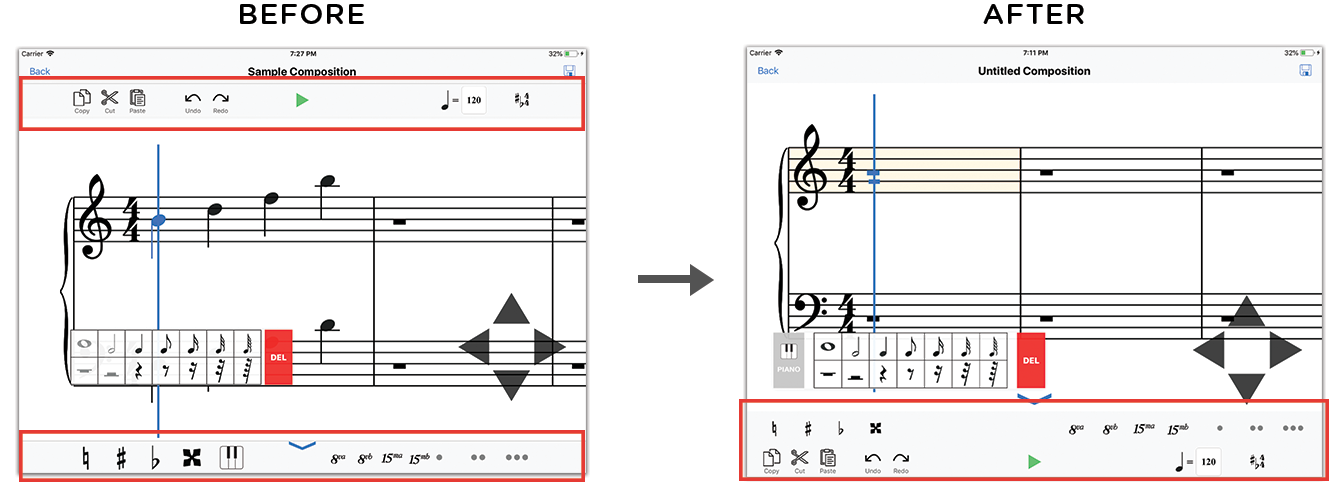
\includegraphics[scale=0.31]{figures/before-after-menu}
				    \caption{The menus before and after changes were made due to the user testing. In the previous iteration, having the menus separated split the focus of the users (see Figure \ref{fig:video_menu}). The top menu was moved to the bottom as well so users would only have to look in one area of the screen.}
				    \label{fig:before-after-menu}
				\end{figure}

				Putting in notes from the keyboard was implemented for this version. However, in the previous version, some of the testers were not able to use the keyboard simply because the show/hide piano button did not seem obvious to them. To resolve this, the piano button was moved to the side of the notation menu to make it more obvious and imply that it is also a method of input (see Figure \ref{fig:before-after-pianobtn}). 

				\begin{figure}[h]
					\centering
					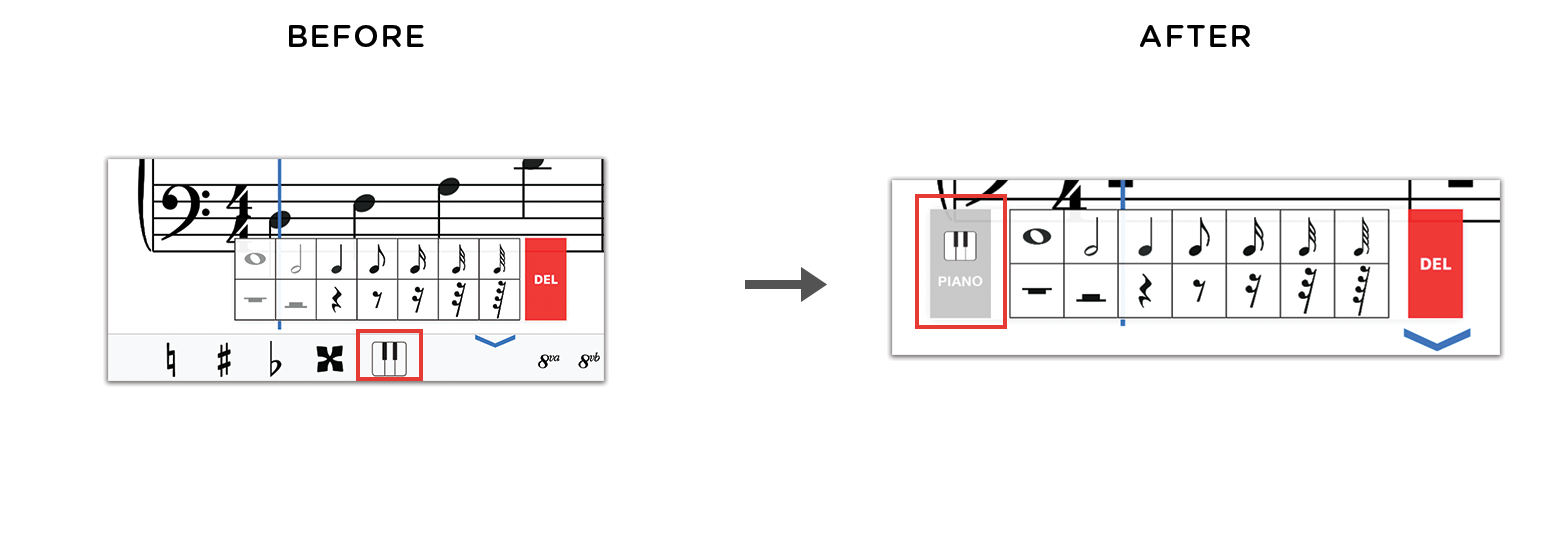
\includegraphics[scale=0.31]{figures/before-after-pianobtn.png}
				    \caption{The show/hide piano button before and after changes were made due to the user testing. In the previous iteration, testers mentioned that the button was not obvious which resulted in them not being able to use the keyboard. The piano button was moved beside the notations menu to make it easier to find.}
				    \label{fig:before-after-pianobtn}
				\end{figure}

				The music playback was also improved since it was the feature with the lowest score in iteration 3, having only 3.1 (see Table \ref{tab:results-features-it3} item 7). The first improvement allowed starting the playback from the current measure the cursor is pointing to. In previous versions, the music playback always started at the first measure, but the testers said that it was quite tedious to have to always start from the first measure especially when they were focusing on editing just a specific part of the composition (see Figure \ref{fig:video_musicplayback}). 

				The visualization of the music playback was also improved. In previous versions, only the current measure was shown which made it harder for composers to find specific notes or rests they felt was off or wanted to change. In this version, the playback was improved to also show the current note or rest that is playing (see Figure \ref{fig:before-after-playback}).

				\begin{figure}[h]
					\centering
					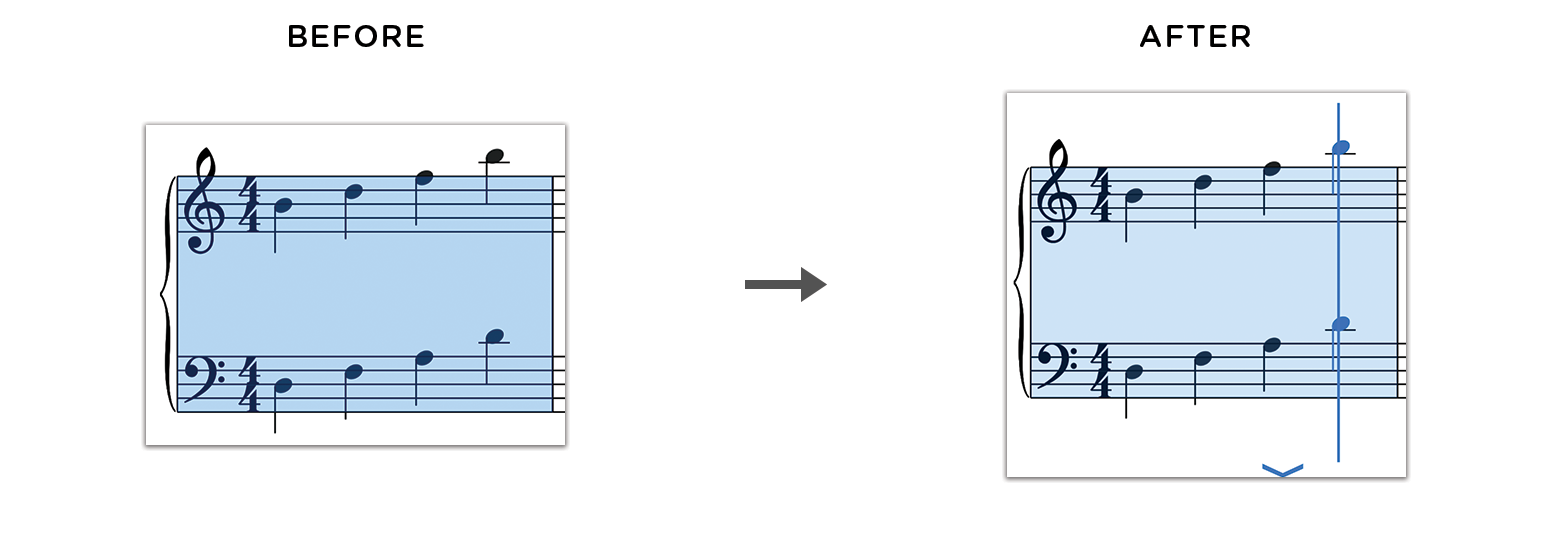
\includegraphics[scale=0.31]{figures/before-after-playback.png}
				    \caption{The music playback before and after changes were made due to the user testing. Previous versions only showed the current measure, making it hard to find specific notes or rests that were off in a measure or melody. The playback was improved to also show the current note/rest that is playing.}
				    \label{fig:before-after-playback}
				\end{figure}

	\section{Verification and Evaluation}
		\subsection{Usability Testing Results}
			This section provides an overview of the results across all iterations. Note that questions for iteration 3 and 4 were different from that of iteration 1 and 2. Despite having different questions, all answers are on a scale of 1 - 4, 1 (Never, Strongly Disagree, or Very Difficult) being the lowest, and 4 (Frequently, Strongly Agree, or Very Easy) being the highest. 

			\subsubsection{Flow Iteration 1} 

				\begin{table}[!htpb]
				  \centering
				  \captionof{table}{Feature Scores per Tester for Iteration 1} \label{tab:results-features-it1}
				  \begin{tabular}{|p{5cm}|R{.7cm}|R{.7cm}|R{.7cm}|R{.7cm}|R{.7cm}|R{1.5cm}|}
				  	\hline
				  	\textbf{Feature} & \textbf{T1} & \textbf{T2} & \textbf{T3} & \textbf{T4} & \textbf{T5} & \textbf{Average} \\ \hline
					Add a Note															& 3.0 & 2.3 & 2.5 & 3.3 & 3.0 & 2.8 \\ \hline 
					Edit a Note 															& 2.5 & 1.5 & 3.0 & 1.8 & 2.0 & 2.2 \\ \hline
					Delete a Note 														& 2.8 & 3.0 & 2.3 & 2.0 & 1.5 & 2.3 \\ \hline
					Move Indicator/Cursor 										& 3.0 & 3.8 & 3.3 & 4.0 & 4.0 & 3.6 \\ \hline
					Move Line/Space Selector 									& 3.3 & 2.5 & 2.8 & 4.0 & 4.0 & 3.3 \\ \hline
					Highlight/Select a Group of Notes 						& 2.8 & 2.5 & 3.3 & 2.5 & 1.3 & 2.5 \\ \hline
					Edit a Highlighted/Selected Group of Notes 		& 3.0 & 2.8 & 2.0 & 2.0 & 1.3 & 2.2 \\ \hline
					Delete a Highlighted/Selected Group of Notes 	& 3.0 & 2.5 & 3.3 & 1.0 & 1.0 & 2.2 \\ \hline

					\multicolumn{6}{|l|}{\textbf{Average}} & 2.6 \\ \hline
				  \end{tabular}
				\end{table}

				From the data gathered and analyzed, a clear difference in respondent sentiment was observed from features that needed note selection versus those that did not. This can be observed in the edit and delete features which had the lowest scores on average. All of these features required the selection feature. All of the respondents were not able to figure out and correctly execute the gesture for selection which was a two-finger drag, which caused some of the poor usability scores given to those features. Although it is common for mobile applications to use one-finger drag to scroll, the results suggest otherwise. It can be noticed in Figure \ref{fig:video_highlight} that the tester was trying to perform the highlight interaction using a one-finger drag which was actually the gesture for the scroll interaction. It was found that the gesture for highlighting (two-finger drag) would have felt more natural if it was switched with the scroll gesture (one-finger drag). Hence, for the second iteration, the gestures for these interactions were switched (see Figure \ref{fig:highlight}).

				\begin{figure}[h]
					\centering
					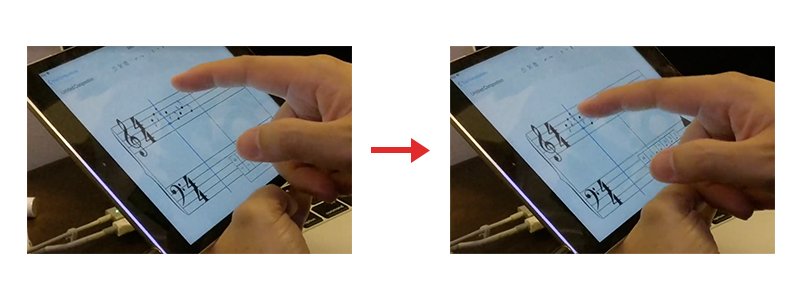
\includegraphics[scale=0.5]{figures/video_highlight.png}
				    \caption{Segments from the user testing video of a tester trying to perform the highlight interaction.}
				    \label{fig:video_highlight}
				\end{figure}

				Other than the note selection feature, respondents have expressed that most of the features worked well and felt comfortable to use. Although it was not like how they would regularly write music (i.e. pen and paper), Flow's method of composing was easy to learn and get used to. Majority liked the ease of using the cursor/indicator because they can simply tap on the location they want or use the arrow keys when they want to be accurate.

			\subsubsection{Flow Iteration 2}
				\begin{longtable}{|p{5cm}|R{.7cm}|R{.7cm}|R{.7cm}|R{.7cm}|R{.7cm}|R{1.5cm}|}
				  \caption{Feature Scores per Tester for Iteration 2} \label{tab:results-features-it2} \\ 
				  	\hline
				  	\textbf{Feature} & \textbf{T1} & \textbf{T2} & \textbf{T3} & \textbf{T4} & \textbf{T5} & \textbf{Average} \\ \hline
					Add a Note 																							& 3.0 & 4.0 & 3.8 & 3.5 & 3.3 & 3.5 \\ \hline
					Delete a Note 																						& 3.5 & 1.8 & 4.0 & 2.5 & 4.0 & 3.2 \\ \hline
					Edit a Note 																							& 3.3 & 3.8 & 4.0 & 2.8 & 4.0 & 3.6 \\ \hline
					Move Position Indicator/Cursor 															& 3.8 & 3.0 & 4.0 & 3.3 & 3.8 & 3.6 \\ \hline
					Move Line/Space Selector 																	& 2.3 & 3.0 & 3.8 & 4.0 & 3.8 & 3.4 \\ \hline
					Highlight/Select a Group of Notes 														& 3.5 & 4.0 & 4.0 & 3.5 & 4.0 & 3.8 \\ \hline
					Edit a Highlighted/Selected Group of Notes 										& 4.0 & 1.8 & 4.0 & 4.0 & 4.0 & 3.6 \\ \hline
					Delete a Highlighted/Selected Group of Notes 									& 4.0 & 4.0 & 4.0 & 4.0 & 4.0 & 4.0 \\ \hline
					Scrolling																								& 3.3 & 3.8 & 3.5 & 3.0 & 3.8 & 3.5 \\ \hline
					Change Time Signature 																		& 3.3 & 1.8 & 3.5 & 3.5 & 3.8 & 3.2 \\ \hline
					Change Key Signature 																		& 3.5 & 4.0 & 3.0 & 3.0 & 4.0 & 3.5 \\ \hline
					Add an Accidental to a Note 																& 4.0 & 4.0 & 4.0 & 3.0 & 4.0 & 3.8 \\ \hline
					Remove an Accidental to a Note 														& 2.0 & 1.3 & 4.0 & 1.8 & 4.0 & 2.6 \\ \hline
					Zooming 																								& 3.3 & 3.3 & 4.0 & 3.0 & 4.0 & 3.5 \\ \hline
					Cut/Copy/Paste a Single Note 															& 4.0 & 2.0 & 4.0 & 1.0 & 4.0 & 3.0 \\ \hline
					Cut/Copy/Paste a Highlighted/Selected Group of Notes 					& 3.8 & 1.8 & 3.0 & 1.0 & 4.0 & 2.7 \\ \hline
					Select a Single Note 																			& 3.5 & 4.0 & 4.0 & 3.0 & 4.0 & 3.7 \\ \hline
					Add an Accidental to a Highlighted/Selected Group of Notes 			& 3.3 & 3.0 & 4.0 & 2.0 & 4.0 & 3.3 \\ \hline
					Remove an Accidental on a Highlighted/Selected Group of Notes 	& 2.0 & 2.5 & 3.0 & 2.0 & 4.0 & 2.7 \\ \hline
					Music Playback 																					& 4.0 & 4.0 & 4.0 & 4.0 & 4.0 & 4.0 \\ \hline

					\multicolumn{6}{|l|}{\textbf{Average}} & 3.4 \\ \hline
				\end{longtable}

				Iteration 2 added some design revisions incorporating the data from the results of iteration 1. The most notable change would be the completely different gesture interaction for highlighting multiple notes. This change resulted in a highlight interaction that not only uses less fingers, but is also less prone to errors. The new interaction influenced most of the results for features involving multiple note selection. Features that scored the lowest like \textit{Edit a Note} and \textit{Delete a Highlighted/Selected Group of Notes} in the first iteration (see Table \ref{tab:results-features-it1} items 2 and 8) scored higher in iteration 2 (see Table \ref{tab:results-features-it2} items 7 and 8). Surprisingly enough, the \textit{Delete a Highlighted/Selected Group of Notes} got the highest score amongst all features aside from the \textit{Music Playback} feature. Again, this can be attributed to the improved highlight and selection interaction. Although a bit subtle, the delete button was also improved during this iteration. Its color was changed to red and it was moved from the bottom of the notation menu to its right side to give it more space. 

				New features were also added in the iteration 2 testing. Given that it was only the first time these were tested, some scored low and were found to need improvement. An example would be the implementation of \textit{Change Time Signature} and \textit{Change Key Signature} (see Table \ref{tab:results-features-it2} items 10 and 11). Both features were quite similar to each other because they utilized a slide interaction. However, the problem with sliders, especially the one for the time signature, was that they had a tendency to be imprecise. This was frustrating for the composers because just slight finger movements would already change the value (see Figure \ref{fig:video_timesig}). If they had a specific value in mind, they needed to be extremely precise and careful when setting the value. On the other hand, the key signature slider was easier, but it only showed a few values at a time so it was sometimes hard for them to find the key signature they wanted. For the succeeding iterations, the menu was changed to allow for easier changing of the time and key signature (see Figure \ref{fig:before-after-tsmenu}).

				\begin{figure}[h]
					\centering
					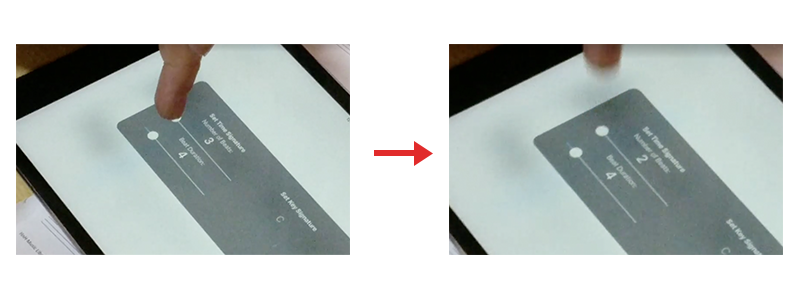
\includegraphics[scale=0.5]{figures/video_timesig.png}
				    \caption{Segments from the user testing video of a tester trying to set a time signature using the menu. It can be noticed that after pointing to the time signature they want, lifting their finger moved the slider to the previous value.}
				    \label{fig:video_timesig}
				\end{figure}

				\begin{figure}[h]
					\centering
					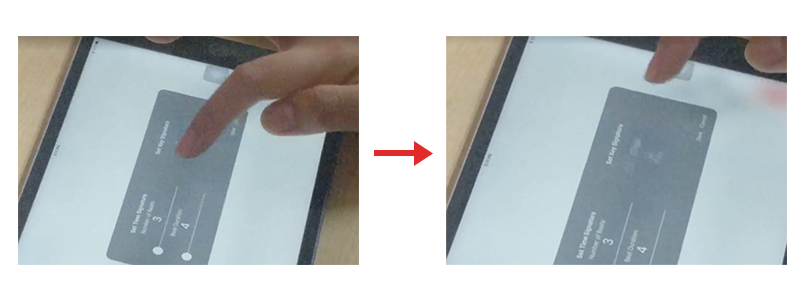
\includegraphics[scale=0.5]{figures/video_keysig.png}
				    \caption{Segments from the user testing video of a tester selecting a key signature using the menu.}
				    \label{fig:video_keysig}
				\end{figure}

				From the observed qualitative data, the transposition interaction was also found to need improvement. In the prototype, users can tap on the up or down arrow keys to instantly transpose the selected notes to a higher or lower pitch respectively. It was observed that this was sometimes confusing and not easy to find (see Figure \ref{fig:video_transpose}). The confusion happened mainly because the users' assumption was that the arrow key was only used to move the cursor and not the notes. They would eventually be able to figure out after some messing around, but this still needed to be improved. Hence, in the succeeding iteration a menu was added containing the transpose arrow keys and other modifiers that would only appear when a user highlights a set of notes (see Figure \ref{fig:before-after-transpose}. This not only made it more obvious, but also saved space by only showing the necessary buttons when needed.

				\begin{figure}[h]
					\centering
					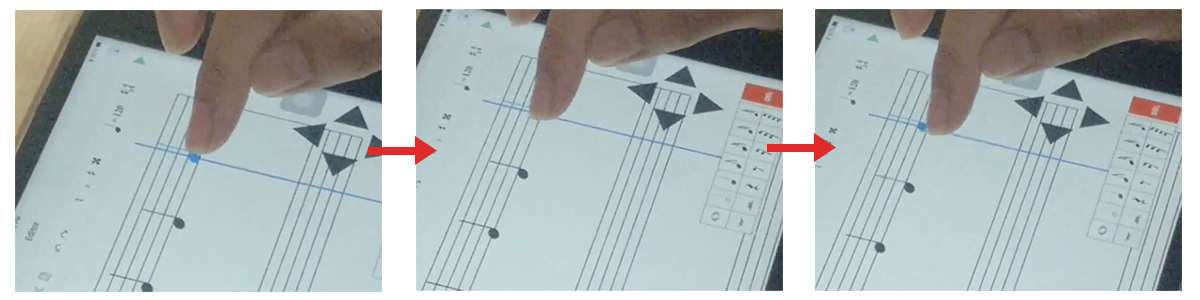
\includegraphics[scale=0.34]{figures/video-transpose.png}
				    \caption{Segments from the user testing video of a tester trying to transpose a note. The tester was trying to drag to transpose and was not able to figure out that they had to use the arrow keys to transpose.}
				    \label{fig:video_transpose}
				\end{figure}

				The \textit{Cut/Copy/Paste} interactions also received some quite low scores (see Table \ref{tab:results-features-it2} items 15 and 16). The main problem with the interaction was the lack of feedback when pressed. The buttons were a bit small and the users had a hard time knowing whether or not they already pressed the button because they could not see any feedback. For the next iteration, the buttons were made a bit bigger and given more space apart. Toast notifications were also added once they successfully executed a cut or copy. 

				The feature that received the lowest score for this iteration was \textit{Remove an Accidental on a Highlighted/Selected Group of Notes}. A lot of the composers said they felt that the buttons were too small and hard to press. However, the main problem with the feature was that the buttons were set up to follow music theory. In music theory, when a sharp is added to a note, it needs to be naturalized to remove the sharp. This was also the logic behind the accidentals in the prototype. When a note has a sharp, the user would have to press the naturalize button to remove it. Unfortunately, this was not obvious to the amateur users. They expected it to be similar to making a text bold or italicized in word processors. What they commonly did was when a note had a sharp, they would press the sharp button again to remove it. Since the buttons were not set up to follow it, nothing would happen and they thought that the buttons did not work. Expert composers, however, did not have a problem using this feature. When asked why they were able to figure it out easily, they mentioned that they just followed music theory. To suit both types of users, the prototype in the succeeding iterations also allowed users to press the accidental button again to remove an already placed accidental aside from the original method of removing accidentals.

			\subsubsection{Flow Iteration 3} % (fold)
			\label{sub:iteration_3}
			
				\begin{landscape}				
					\begin{longtable}{|p{3.5cm}|R{.7cm}|R{.7cm}|R{.7cm}|R{.7cm}|R{.7cm}|R{.7cm}|R{.7cm}|R{.7cm}|R{.7cm}|R{.7cm}|R{.7cm}|R{.7cm}|R{.7cm}|R{.7cm}|R{.7cm}|R{1.5cm}|}
						\caption{Feature Scores per Tester for Iteration 3} \label{tab:results-features-it3} \\
						  	\hline
						  	\textbf{Feature} & \textbf{T1} & \textbf{T2} & \textbf{T3} & \textbf{T4} & \textbf{T5} & \textbf{T6} & \textbf{T7} & \textbf{T8} & \textbf{T9} & \textbf{T10} & \textbf{T11}& \textbf{T12} & \textbf{T13} & \textbf{T14} & \textbf{T15} & \textbf{Average} \\ \hline
							
						  	Select or highlight notes/chords 		& 4.0 & 4.0 & 3.5 & 4.0 & 3.5 & 3.0 & 3.5 & 4.0 & 3.5 & 3.0 & 4.0 & 4.0 & 4.0 & 3.5 & 3.5 & 3.7 \\ \hline
							Add notes/chords 							& 4.0 & 4.0 & 3.5 & 4.0 & 3.0 & 3.0 & 4.0 & 3.5 & 4.0 & 3.0 & 4.0 & 4.0 & 4.0 & 4.0 & 4.0 & 3.7 \\ \hline
							Edit notes/chords 							& 4.0 & 4.0 & 3.0 & 4.0 & 2.0 & 2.5 & 3.5 & 2.0 & 2.5 & 3.0 & 4.0 & 4.0 & 3.5 & 4.0 & 3.0 & 3.3 \\ \hline
							Delete notes/chords 						& 4.0 & 4.0 & 4.0 & 4.0 & 3.0 & 2.5 & 4.0 & 3.5 & 3.0 & 3.0 & 4.0 & 4.0 & 4.0 & 4.0 & 4.0 & 3.7 \\ \hline
							Cut, copy, or paste notes/chords 	& 1.0 & 4.0 & 4.0 & 4.0 & 3.5 & 3.0 & 1.5 & 3.5 & 4.0 & 3.0 & 4.0 & 3.5 & 4.0 & 4.0 & 3.0 & 3.3 \\ \hline
							Undo/redo an action 						& 4.0 & 3.0 & 3.5 & 4.0 & 3.5 & 4.0 & 4.0 & 3.5 & 4.0 & 4.0 & 4.0 & 4.0 & 4.0 & 4.0 & 4.0 & 3.8 \\ \hline
							Music Playback 								& 1.0 & 4.0 & 3.0 & 4.0 & 3.0 & 3.5 & 3.0 & 3.0 & 3.0 & 3.5 & 2.0 & 4.0 & 3.0 & 3.0 & 3.0 & 3.1 \\ \hline

							\multicolumn{16}{|l|}{\textbf{Average}} & 3.5 \\ \hline

					\end{longtable}
				\end{landscape}

				\begin{comment}
					Changes for iteration 3:

						Written about:
							Menu shows all options, just disables them when not needed
							Revised show menu button
							Transpose hovered notes, not just selected
							Moved menu to bottom
							Input from keyboard
							Moved piano button


						Playback from the start of cursor
						Playback shows current note/rest playing
						
						Draggable cursor

				\end{comment}

				The problems that were found in iteration 2 were solved in iteration 3. In iteration 2, the overall edit feature only had a score of 3.2 (see Table \ref{tab:results-features-it2} item 3). But in iteration 3, the average score increased to 3.3 (see Table \ref{tab:results-features-it3} item 3). From the observed qualitative results, adding and removing accidentals were now easier for the testers. The separate transpose button also made the transpose feature clearer for them. Most of the issues with this iteration however, came from the placing and visibility of the other features. 

				%The problems that were found in iteration 2 were solved in iteration 3. In iteration 2, the overall edit feature only had a score of 3.2 (see Table \ref{tab:common-samples-it2} item 3). But for the same testers in iteration 3, the average score increased to 3.6 (see Table \ref{tab:common-samples-it3} item 3) while for all testers, the average score is 3.3 (see Table \ref{tab:results-features-it3} item 3). From the observed qualitative results, adding and removing accidentals were now easier for the testers. The separate transpose button also made the transpose feature clearer for them. Most of the issues with this iteration however, came from the placing and visibility of the other features. 

				Since a lot of the testers from iteration 2 expressed their opinion that the menu felt a bit cramped and the buttons a bit small, a separate menu was created and placed at the bottom of the screen. This menu contained modifiers like the accidentals and dots. This menu's visibility could be toggled using show/hide buttons. However, one issue that was observed was that the show button was not that obvious. Because of this, some users were not able to access the other modifiers because they were not able to see the menu. This was solved for the next iteration by revising the show button. 

				However, notice that testers 1 and 7 rated the \textit{Cut, copy, or paste notes/chords} feature quite low at 1.0 and 1.5 respectively. When asked why, they said that they could not figure out how to do it immediately because they were not able to find the icons easily. This relates to another issue with the bottom menu was that it split the focus of the users. Since there was now a menu at the top and a menu at the bottom, some users had a harder time finding specific functions. Their initial instinct was to first look at the bottom menu so it added extra load just to find the top menu functions like cut, copy, or paste (see Figure \ref{fig:video_menu}). For the next iteration, the top menu was moved to the bottom so users would only have to look in one segment (see Figure \ref{fig:before-after-menu}). 

				\begin{figure}[h]
					\centering
					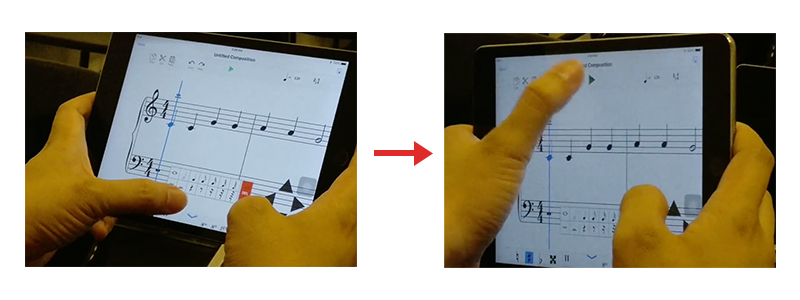
\includegraphics[scale=0.5]{figures/video_menu.png}
				    \caption{Segments from the user testing video of a tester looking for the play button in the bottom menu.}
				    \label{fig:video_menu}
				\end{figure}

				It was also mentioned that for iteration 3, a new menu containing the transpose arrow keys and modifiers like retrograde and slur was added. To prevent cramming the screen, this menu was only made to show when needed which was when users highlighted a group of notes. The problem with this was that users did not usually follow that line of thinking. They did not highlight first then select the modifier, they expected it to be the other way around. For example, they wanted to create a slur, they would try to find the button first then pick notes to slur after. This resulted in them thinking that those functions were not available. For the next iteration, the menu was no longer hidden. It always showed even when just hovering on a note but disabled the modifiers that were not valid. 

				Iteration 3 also added a keyboard so users can try out melodies before inputting them on the digital sheet. However, users also expressed that they wanted to be able to input from the keyboard so it was added for iteration 4. However, it was also observed that some users were not able to find the button that showed the keyboard. Although it had a button at the bottom menu, it was not that obvious to the users since they were focused on the notation controls menu. The button was then moved beside the notations menu for the next iteration (see Figure \ref{fig:before-after-pianobtn}). 

				From the quantitative results, it can be seen that the \textit{Music Playback} scored the lowest. Note that tester 1 gave the feature a score of only 1.0. This happened because of two reasons: (1) the playback always started from the first measure, and (2) the playback did not show the current note/rest that was playing. Observations made during the tests showed that the composers would usually place the cursor at the measure where they wanted to start playing from. They would be surprised to find out that the playback always started from the first measure, regardless of the cursor placement (see Figure \ref{fig:video_musicplayback}). This feature was incorporated in iteration 4 to reduce the tediousness when writing a long composition. Another issue related to the playback was that it only showed the current measure that was playing and not the current note/rest. This was also added for iteration 4 to reduce confusion and to make it easier to find the notes/rests they need to change in case they want to modify the melody (see Figure \ref{fig:before-after-playback}). 

				\begin{figure}[H]
					\centering
					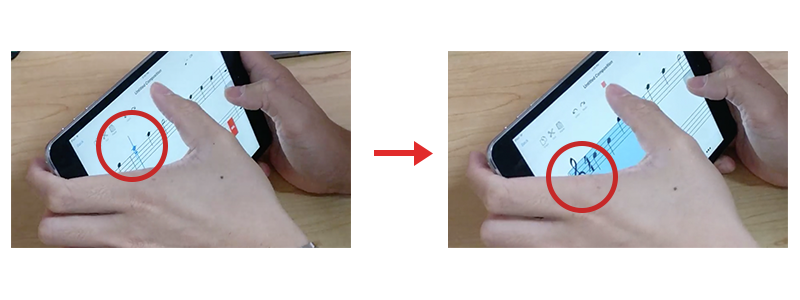
\includegraphics[scale=0.5]{figures/video_musicplayback.png}
				    \caption{Segments from the user testing video of a tester trying to start the playback from a specific measure.}
				    \label{fig:video_musicplayback}
				\end{figure}
			% subsection iteration_3 (end)

			\subsubsection{Flow Iteration 4} % (fold)
			\label{sub:iteration_4}

				 \begin{landscape}				
					\begin{longtable}{|p{3.5cm}|R{.7cm}|R{.7cm}|R{.7cm}|R{.7cm}|R{.7cm}|R{.7cm}|R{.7cm}|R{.7cm}|R{.7cm}|R{.7cm}|R{.7cm}|R{1.5cm}|}
						\caption{Feature Scores per Tester for Iteration 4} \label{tab:results-features-it4} \\
						  	\hline
						  	\textbf{Feature} & \textbf{T1} & \textbf{T2} & \textbf{T3} & \textbf{T4} & \textbf{T5} & \textbf{T6} & \textbf{T7} & \textbf{T8} & \textbf{T9} & \textbf{T10} & \textbf{T11} & \textbf{Average} \\ \hline

						  	Select or highlight notes/chords 		& 3.0 & 1.3 & 4.0 & 3.7 & 4.0 & 3.7 & 3.7 & 3.3 & 3.0 & 4.0 & 4.0 & 3.4 \\ \hline
							Add notes/chords 							& 2.7 & 2.3 & 4.0 & 2.7 & 3.0 & 3.0 & 4.0 & 3.3 & 2.7 & 4.0 & 4.0 & 3.2 \\ \hline
							Edit notes/chords 							& 2.7 & 2.7 & 3.7 & 2.7 & 2.3 & 2.3 & 3.7 & 3.3 & 3.0 & 4.0 & 2.3 & 3.0 \\ \hline
							Delete notes/chords 						& 4.0 & 3.0 & 4.0 & 4.0 & 3.3 & 2.7 & 4.0 & 3.3 & 1.7 & 3.7 & 4.0 & 3.4 \\ \hline
							Cut, copy, or paste notes/chords 	& 3.3 & 1.0 & 3.7 & 3.7 & 4.0 & 2.0 & 4.0 & 3.3 & 2.7 & 3.0 & 1.3 & 2.9 \\ \hline
							Undo/redo an action 						& 4.0 & 3.3 & 4.0 & 4.0 & 3.7 & 3.0 & 4.0 & 4.0 & 1.7 & 4.0 & 4.0 & 3.6 \\ \hline
							Music Playback 								& 3.0 & 2.3 & 2.0 & 2.7 & 3.7 & 4.0 & 3.0 & 4.0 & 1.0 & 2.3 & 4.0 & 2.9 \\ \hline

							\multicolumn{12}{|l|}{\textbf{Average}} & 3.2 \\ \hline

					\end{longtable}
				\end{landscape} 

				In iteration 4, most of the testers felt that Flow was a bit lacking in terms of features and modifiers, which was understandable given that not all musical notation modifiers were implemented to give focus to the interaction. However, some did enjoy the method of interaction, specifically the presence of the cursor, and commented that it was straightforward and easy to understand immediately. 

				It can be seen, however, that tester 1 rated the \textit{Select or highlight notes/chords} and \textit{Cut, copy, or paste notes/chords} features quite low. The reason why these two are low are actually connected. The said tester was not actually able to figure out how to perform the highlight gesture. Because of that, they were also not able to fully perform cut/copy/paste actions because they could not highlight any notes/rests. However, they also mentioned that they were not really accustomed to using mobile applications which most likely caused the unfamiliarity with the gesture. 

				It can also be noticed that tester 9 rated the \textit{Music playback} feature very low at 1.0. This was caused by a bug in the application that would play the tempo of the composition slower than it should be. This only happened when the user would play the composition repeatedly. An inefficient piece of code caused a variable to be instantiated repeatedly, causing the playback to slow down after multiple playback attempts. 
			
			% subsection iteration_4 (end)

		\subsection{Comparative Analysis Between Iterations} % (fold)
		\label{sec:comparative_analysis}

			Shown in Table \ref{tab:summarized-all} and Figures \ref{fig:select-bar}, \ref{fig:add-bar}, \ref{fig:edit-bar}, and \ref{fig:delete-bar} are the per feature summarized scores across all iterations. It can be observed that each feature increases in its average rating from iteration 1 to iteration 3. This can imply an improvement in the user experience. Scores went down a bit in iteration 4, but this could probably be attributed to the demographics of the testers since all but one (1) have never used the application before and most were experts. The greatest increase however, comes from iteration 1 to iteration 2, with a total increase of 3.6 and an average increase of 0.9. 

			\begin{table}[H]
			  \centering
			  \captionof{table}{Summarized Feature Scores from Iteration 1 - 4} \label{tab:summarized-all}
			  \begin{tabular}{|p{2.7cm}|R{.7cm}|R{.7cm}|R{.7cm}|R{.7cm}|R{.5cm}|R{1.4cm}|R{1.4cm}|R{1.4cm}|}
			  	\hline
			  	\textbf{Feature} & \textbf{I1} & \textbf{I2} & \textbf{I3} & \textbf{I4} & \begin{math}\bm{\mu}\end{math} & \textbf{I2 - I1} & \textbf{I3 - I2} & \textbf{I4 - I3} \\ \hline

			  	Select or highlight notes/chords 	& 3.1 & 3.6 & 3.7 & 3.4 & 3.4 & 0.5 & 0.1 & -0.3 \\ \hline
				Add notes/chords 						& 2.8 & 3.5 & 3.7 & 3.2 & 3.3 & 0.7 & 0.2 & -0.5 \\ \hline
				Edit notes/chords 						& 2.2 & 3.2 & 3.3 & 3.0 & 2.9 & 1.0 & 0.1 & -0.3 \\ \hline
				Delete notes/chords 					& 2.2 & 3.6 & 3.7 & 3.4 & 3.2 & 1.4 & 0.1 & -0.3 \\ \hline

			  \end{tabular}
			\end{table}

			\begin{figure}[H]
				\centering
				\frame{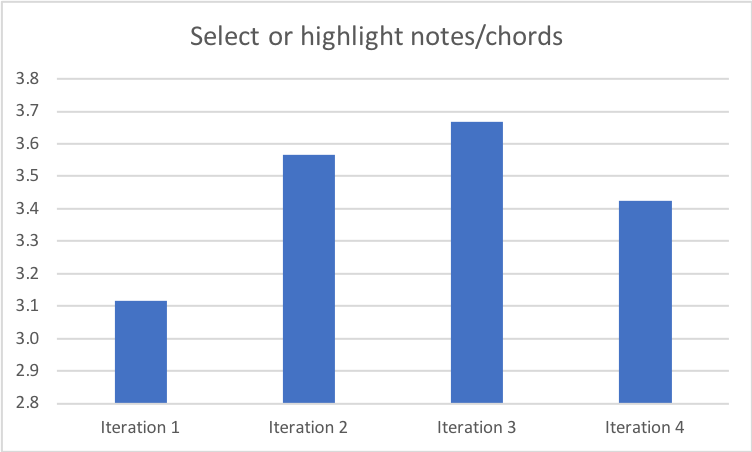
\includegraphics[scale=0.7]{figures/results-select-bar.png}}
			    \caption{Bar chart showing the summarized feature scores of the \textit{Select or highlight notes/chords} feature from iteration 1 to iteration 4.}
			    \label{fig:select-bar}
			\end{figure} 

			\begin{figure}[H]
				\centering
				\frame{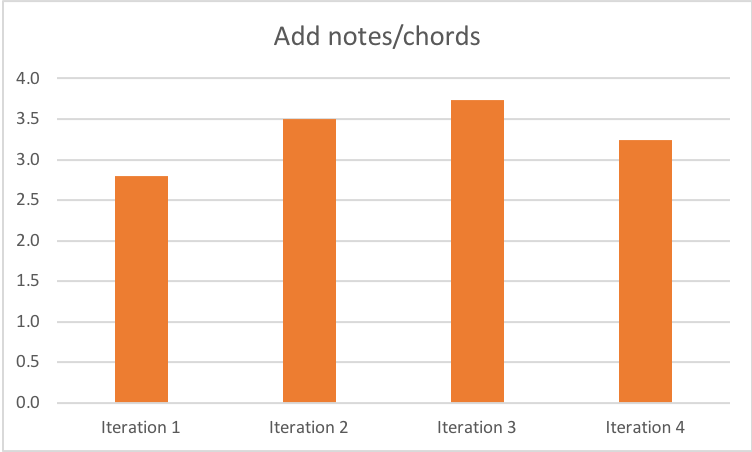
\includegraphics[scale=0.7]{figures/results-add-bar.png}}
			    \caption{Bar chart showing the summarized feature scores of the \textit{Add notes/chords} feature from iteration 1 to iteration 4.}
			    \label{fig:add-bar}
			\end{figure} 

			\begin{figure}[H]
				\centering
				\frame{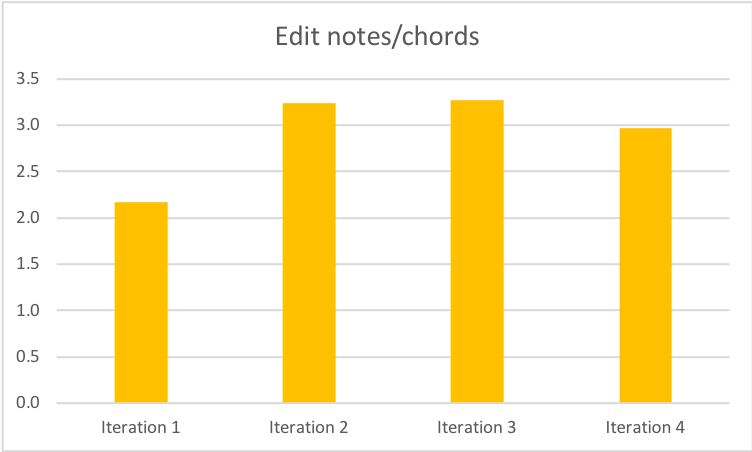
\includegraphics[scale=0.7]{figures/results-edit-bar.png}}
			    \caption{Bar chart showing the summarized feature scores of the \textit{Edit notes/chords} feature from iteration 1 to iteration 4.}
			    \label{fig:edit-bar}
			\end{figure} 


			\begin{figure}[H]
				\centering
				\frame{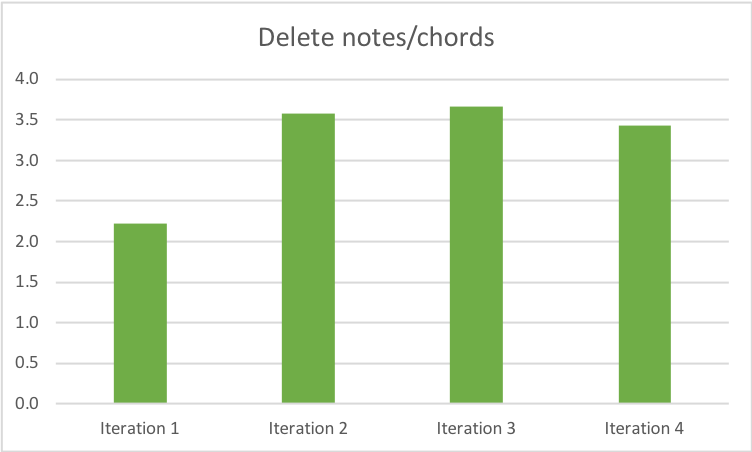
\includegraphics[scale=0.7]{figures/results-delete-bar.png}}
			    \caption{Bar chart showing the summarized feature scores of the \textit{Delete notes/chords} feature from iteration 1 to iteration 4.}
			    \label{fig:delete-bar}
			\end{figure} 

			The feature with the greatest increase is the delete function. It started as one of the features with the lowest score in iteration 1 at only 2.2 and ended up as the feature with one of the highest scores in iteration 4 at 3.4. This is because of the several improvements made to the interaction of the delete feature. In iteration 1, users would have to use the highlight feature to delete, even if it was just a single note/rest. With the changes made to the highlight interaction and allowing users to delete when the cursor is pointed on the note/rest, the experience of deleting and even editing improved for the users. The delete feature was still further improved for iteration 3 by allowing users to delete even when the cursor is not exactly pointed on the note/rest, as long as the cursor is on the same x-coordinate and staff as the note. 

			\begin{comment}
			The five (5) testers present in iteration 1 and 2 were also present in iteration 3. This was done to allow an analysis of common samples and see if there was an improvement in the user experience for these testers. Tables \ref{tab:common-samples-it1}, \ref{tab:common-samples-it2}, and \ref{tab:common-samples-it3} show the scores given by these testers for similar features from iteration 1, 2, and 3 respectively. Note that for iteration 1 and 2, since the features were more specific, similar features were grouped into a more general description of the feature to match that of iteration 3. The average of the scores from the similar features was the score used for the general feature.

			\begin{table}[!htpb]
			  \centering
			  \captionof{table}{Common Samples Feature Scores for Iteration 1} \label{tab:common-samples-it1}
			  \begin{tabular}{|p{3cm}|R{.7cm}|R{.7cm}|R{.7cm}|R{.7cm}|R{.7cm}|R{.8cm}|R{.8cm}|R{.8cm}|R{.8cm}|}
			  	\hline
			  	\textbf{Feature} & \textbf{T1} & \textbf{T2} & \textbf{T3} & \textbf{T4} & \textbf{T5} & \begin{math}\bm{\mu}\end{math} & \textbf{min} & \textbf{max} & \begin{math}\bm{\sigma}\end{math} \\ \hline

			  	Select or highlight notes/chords 	& 3.0 & 3.1 & 3.1 & 3.5 & 2.9 & 3.1 & 2.9 & 3.5 & 0.2 \\ \hline
				Add notes/chords 						& 3.0 & 2.5 & 3.0 & 3.3 & 2.3 & 2.8 & 2.3 & 3.3 & 0.4 \\ \hline
				Edit notes/chords 						& 2.8 & 2.5 & 1.6 & 1.9 & 2.1 & 2.2 & 1.6 & 2.8 & 0.5 \\ \hline
				Delete notes/chords 					& 2.9 & 2.8 & 1.3 & 1.5 & 2.8 & 2.2 & 1.3 & 2.9 & 0.8 \\ \hline
				

			  \end{tabular}
			\end{table}

			\begin{table}[!htpb]
			  \centering
			  \captionof{table}{Common Samples Feature Scores for Iteration 2} \label{tab:common-samples-it2}
			  \begin{tabular}{|p{3cm}|R{.7cm}|R{.7cm}|R{.7cm}|R{.7cm}|R{.7cm}|R{.8cm}|R{.8cm}|R{.8cm}|R{.8cm}|}
			  	\hline
			  	\textbf{Feature} & \textbf{T1} & \textbf{T2} & \textbf{T3} & \textbf{T4} & \textbf{T5} & \begin{math}\bm{\mu}\end{math} & \textbf{min} & \textbf{max} & \begin{math}\bm{\sigma}\end{math} \\ \hline

			  	Select or highlight notes/chords 	& 3.8 & 3.9 & 3.6 & 3.3 & 3.2 & 3.6 & 3.2 & 3.9 & 0.3 \\ \hline
				Add notes/chords 						& 3.3 & 3.8 & 3.5 & 4.0 & 3.0 & 3.5 & 3.0 & 4.0 & 0.4 \\ \hline
				Edit notes/chords 						& 4.0 & 3.8 & 2.6 & 2.7 & 3.1 & 3.2 & 2.6 & 4.0 & 0.6 \\ \hline
				Delete notes/chords 					& 4.0 & 4.0 & 3.3 & 2.9 & 3.8 & 3.6 & 2.9 & 4.0 & 0.5 \\ \hline
				

			  \end{tabular}
			\end{table}

			\begin{table}[H]
			  \centering
			  \captionof{table}{Common Samples Feature Scores for Iteration 3} \label{tab:common-samples-it3}
			  \begin{tabular}{|p{3cm}|R{.7cm}|R{.7cm}|R{.7cm}|R{.7cm}|R{.7cm}|R{.8cm}|R{.8cm}|R{.8cm}|R{.8cm}|}
			  	\hline
			  	\textbf{Feature} & \textbf{T1} & \textbf{T2} & \textbf{T3} & \textbf{T4} & \textbf{T5} & \begin{math}\bm{\mu}\end{math} & \textbf{min} & \textbf{max} & \begin{math}\bm{\sigma}\end{math} \\ \hline

			  	Select or highlight notes/chords 	& 3.5 & 4.0 & 3.5 & 4.0 & 4.0 & 3.8 & 3.5 & 4.0 & 0.3 \\ \hline
				Add notes/chords 						& 3.5 & 4.0 & 4.0 & 4.0 & 4.0 & 3.9 & 3.5 & 4.0 & 0.2 \\ \hline
				Edit notes/chords 						& 3.0 & 4.0 & 3.0 & 4.0 & 4.0 & 3.6 & 3.0 & 4.0 & 0.5 \\ \hline
				Delete notes/chords 					& 4.0 & 4.0 & 4.0 & 4.0 & 4.0 & 4.0 & 4.0 & 4.0 & 0.0 \\ \hline

			  \end{tabular}
			\end{table}

			Shown in Table \ref{tab:summarized-common-samples} and Figures \ref{fig:select-line}, \ref{fig:add-line}, \ref{fig:edit-line}, and \ref{fig:delete-line} are the per feature summarized scores from the common samples. It can be observed that each feature increases in its average rating per iteration. This can imply an increase in the user experience for the common samples. The greatest increase however, comes from iteration 1 to iteration 2, with a total increase of 3.6 and an average increase of 0.9. For iteration 2 to iteration 3, it was only a 1.4 total increase and an average increase of 0.4 but is still an improvement. 

			\begin{table}[H]
			  \centering
			  \captionof{table}{Summarized Common Samples Feature Scores from Iteration 1 - 3} \label{tab:summarized-common-samples}
			  \begin{tabular}{|p{4cm}|R{.7cm}|R{.7cm}|R{.7cm}|R{.7cm}|R{1.5cm}|R{1.5cm}|}
			  	\hline
			  	\textbf{Feature} & \textbf{I1} & \textbf{I2} & \textbf{I3} & \begin{math}\bm{\mu}\end{math} & \textbf{I2 - I1} & \textbf{I3 - I2} \\ \hline

			  	Select or highlight notes/chords 	& 3.1 & 3.6 & 3.8 & 3.5 & 0.5 & 0.2 \\ \hline
				Add notes/chords 						& 2.8 & 3.5 & 3.9 & 3.4 & 0.7 & 0.4 \\ \hline
				Edit notes/chords 						& 2.2 & 3.2 & 3.6 & 3.0 & 1.1 & 0.4 \\ \hline
				Delete notes/chords 					& 2.2 & 3.6 & 4.0 & 3.3 & 1.4 & 0.4 \\ \hline
			  	
			  \end{tabular}
			\end{table}

			\begin{figure}[H]
				\centering
				\frame{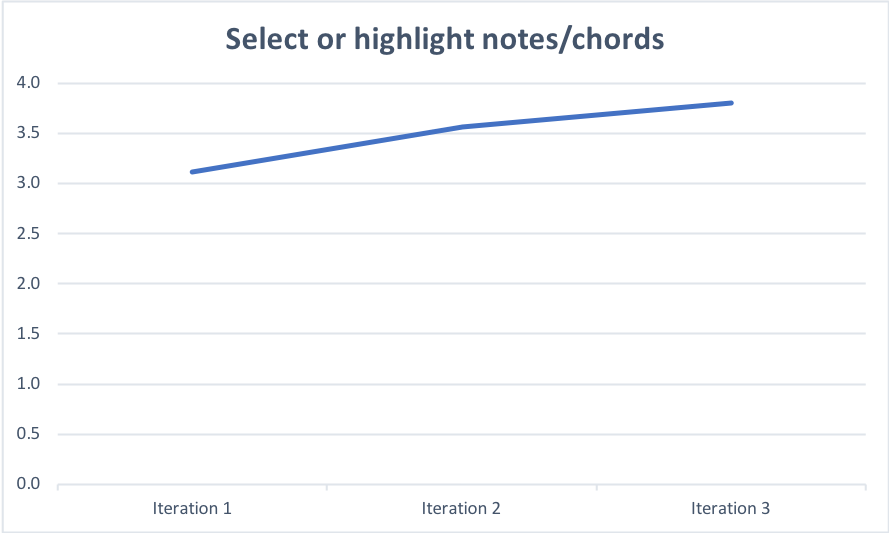
\includegraphics[scale=0.7]{figures/select-line.png}}
			    \caption{Line chart showing the summarized common samples feature scores of the \textit{Select or highlight notes/chords} feature from iteration 1 to iteration 3.}
			    \label{fig:select-line}
			\end{figure} 

			\begin{figure}[H]
				\centering
				\frame{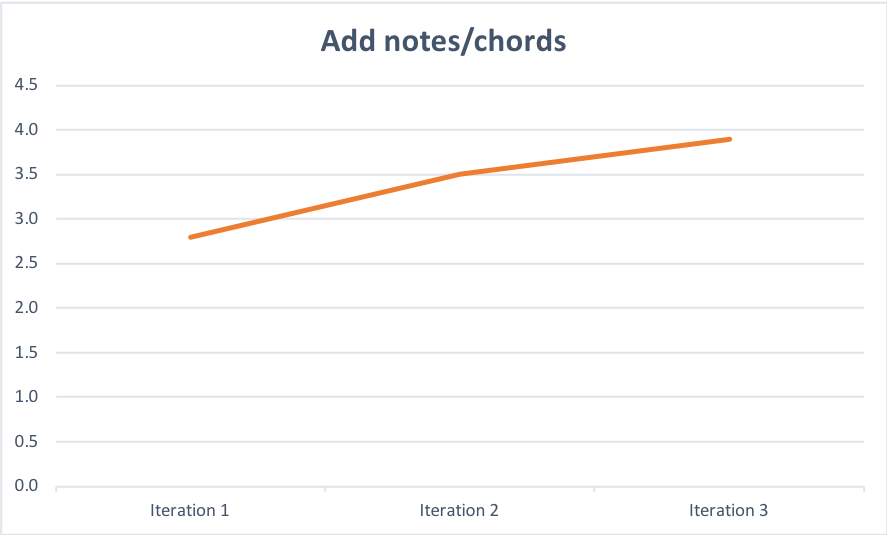
\includegraphics[scale=0.7]{figures/add-line.png}}
			    \caption{Line chart showing the summarized common samples feature scores of the \textit{Add notes/chords} feature from iteration 1 to iteration 3.}
			    \label{fig:add-line}
			\end{figure} 

			\begin{figure}[H]
				\centering
				\frame{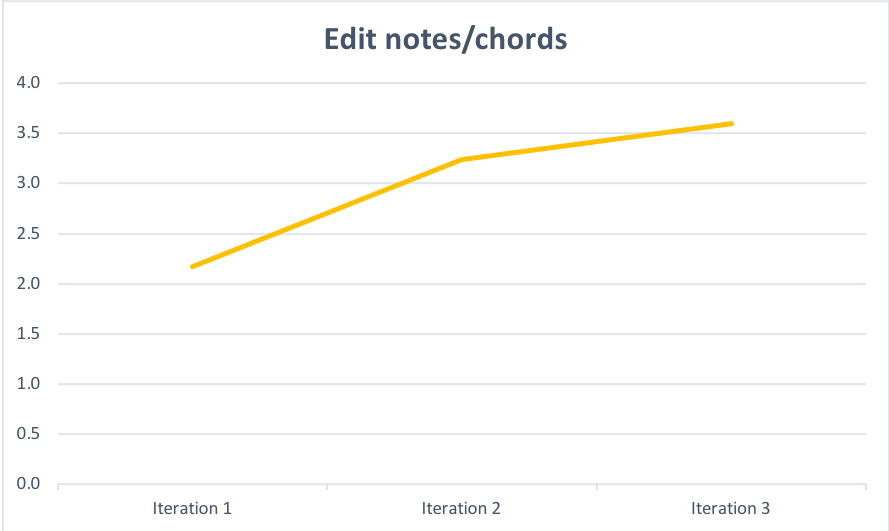
\includegraphics[scale=0.7]{figures/edit-line.png}}
			    \caption{Line chart showing the summarized common samples feature scores of the \textit{Edit notes/chords} feature from iteration 1 to iteration 3.}
			    \label{fig:edit-line}
			\end{figure} 


			\begin{figure}[H]
				\centering
				\frame{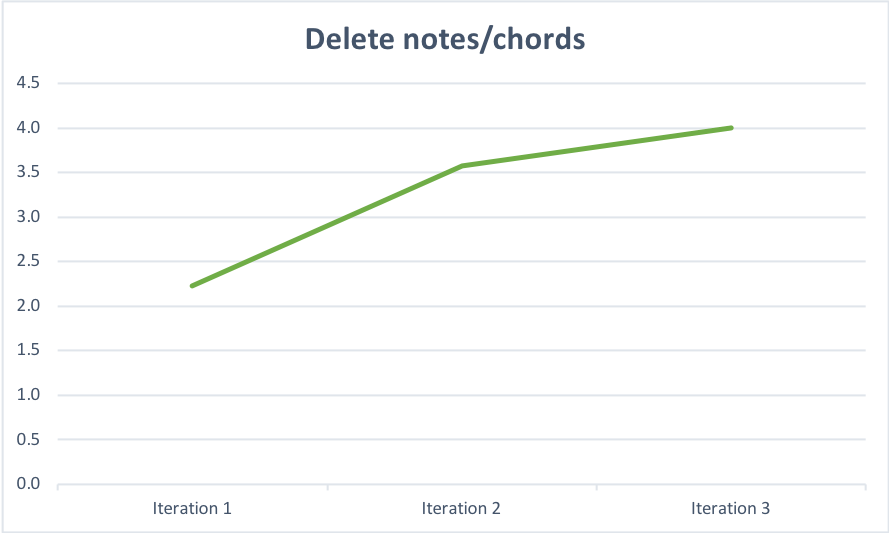
\includegraphics[scale=0.7]{figures/delete-line.png}}
			    \caption{Line chart showing the summarized common samples feature scores of the \textit{Delete notes/chords} feature from iteration 1 to iteration 3.}
			    \label{fig:delete-line}
			\end{figure} 
			
			The feature with the greatest increase from iteration 1 to iteration 3 is the delete function. It started as one of the features with the lowest score in iteration 1 at only 2.2 and ended up as the feature with the highest score in iteration 3 at a perfect 4.0, having a total increase of 1.8 points. This can be attributed to the several improvements made to the interaction of the delete feature. In iteration 1, users would have to use the highlight feature to delete, even if it was just a single note/rest. With the changes made to the highlight interaction and allowing users to delete when the cursor is pointed on the note/rest, the experience of deleting and even editing improved for the users. The delete feature was still further improved for iteration 3 by allowing users to delete even when the cursor is not exactly pointed on the note/rest, as long as the cursor is on the same x-coordinate and staff as the note. 

			\end{comment}

			% Compare the alpha level you chose (i.e. 0.05) to the p-value in the output. If the p-value in the output is smaller than the alpha level you chose, reject the null hypothesis.

			\begin{comment}
			Since there were also some new testers introduced in iteration 3, it would also be possible to compare these ``isolates'' with the common samples. Tables \ref{tab:compare-cs-is} and \ref{tab:compare-i3-is} show the comparison of the scores from the common samples (across all iterations and iteration 3 only) versus the isolates. A two-way t-test was also performed with the null hypothesis being the two having a mean of zero (0) or having no significant difference, and with the alpha set to 0.05.

			Notice that in Table \ref{tab:compare-cs-is}, the case where the average scores across all iterations were used in comparison to the scores given by the isolates, the isolates had higher scores in all features. This is mainly because of the lower scores from the previous two iterations. A lot of improvements were needed, hence they pulled down the scores for the common samples across all iterations. However, the opposite is true when only the scores from iteration 3 are compared with the scores from the isolates. This was likely to happen since the common samples already had experience using the application beforehand and knew what to expect while the isolates were entirely new to the application. In both cases, the p-value is less than the alpha, which means that the null hypothesis is rejected and that there is a significant difference. 

			\begin{table}[H]
			  \centering
			  \captionof{table}{Comparison of the Common Samples Across All Iterations versus the Isolates from Iteration 3} \label{tab:compare-cs-is}
			  \begin{tabular}{|p{5cm}|R{2.5cm}|R{2.5cm}|}
			  	\hline
			  	\textbf{Feature} & \textbf{Common Samples} & \textbf{Isolates} \\ \hline

			  	Select or highlight notes/chords 			& 3.49 & 3.60 \\ \hline
				Add notes/chords 								& 3.40 & 3.65 \\ \hline
				Edit notes/chords 								& 3.01 & 3.10 \\ \hline
				Delete notes/chords 							& 3.27 & 3.50 \\ \hline

				\begin{math}\bm{\mu}\end{math} 		& 3.29 & 3.46 \\ \hline
				\begin{math}\bm{\sigma}\end{math} 	& 0.21 & 0.25 \\ \hline

				\textbf{alpha} 										& \multicolumn{2}{r|}{0.05} \\ \hline
			  	\textbf{p-value} 									& \multicolumn{2}{r|}{0.01} \\ \hline
			  \end{tabular}
			\end{table}

			\begin{table}[H]
			  \centering
			  \captionof{table}{Comparison of the Common Samples from Iteration 3 versus the Isolates from Iteration 3} \label{tab:compare-i3-is}
			  \begin{tabular}{|p{5cm}|R{2.5cm}|R{2.5cm}|}
			  	\hline
			  	\textbf{Feature} & \textbf{Iteration 3} & \textbf{Isolates} \\ \hline

			  	Select or highlight notes/chords 			& 3.80 & 3.60 \\ \hline
				Add notes/chords 								& 3.90 & 3.65 \\ \hline
				Edit notes/chords 								& 3.60 & 3.10 \\ \hline
				Delete notes/chords 							& 4.00 & 3.50 \\ \hline

				\begin{math}\bm{\mu}\end{math} 		& 3.83 & 3.46 \\ \hline
				\begin{math}\bm{\sigma}\end{math} 	& 0.17 & 0.25 \\ \hline

				\textbf{alpha} 										& \multicolumn{2}{r|}{0.05} \\ \hline
			  	\textbf{p-value} 									& \multicolumn{2}{r|}{0.01} \\ \hline
			  \end{tabular}
			\end{table}

			% Here
			The scores from the common samples may also be compared with the scores from the control group from iteration 4. Like the isolates, the control group is also made up of composers who have never used the application before, but this time, majority of them are experts. Table \ref{tab:compare-cs-cg} shows their comparison against the scores from the common samples across all iterations while Table \ref{tab:compare-i3-cg} shows their comparison against the scores from the common samples in iteration 3 only. Similar to the isolates, a two-way t-test was also performed with the null hypothesis being the two having a mean of zero (0) or having no significant difference, and with the alpha set to 0.05.

			It is not surprising to see that in both cases, the control group had the lower score on average. Given that most of the testers were experts, they had higher expectations and were a lot more strict in rating the application. A lot of them also felt Flow lacked in the number of features and modifiers it offered, hence the somewhat low scores, especially with the edit feature. Notice that for the common samples across all iterations versus the control group, the p-value was higher than the alpha, which means there is no significant difference between the two. On the other hand, when only the iteration 3 scores from the common samples are compared with the control group, the p-value is lower than the alpha hence there is a significant difference between them. 

			\begin{table}[H]
			  \centering
			  \captionof{table}{Comparison of the Common Samples Across All Iterations versus the Control Group from Iteration 4} \label{tab:compare-cs-cg}
			  \begin{tabular}{|p{5cm}|R{2.5cm}|R{2.5cm}|}
			  	\hline
			  	\textbf{Feature} & \textbf{Common Samples} & \textbf{Control Group} \\ \hline

			  	Select or highlight notes/chords 			& 3.49 & 3.37 \\ \hline
				Add notes/chords 								& 3.40 & 3.17 \\ \hline
				Edit notes/chords 								& 3.01 & 2.87 \\ \hline
				Delete notes/chords 							& 3.27 & 3.40 \\ \hline

				\begin{math}\bm{\mu}\end{math} 		& 3.29 & 3.20 \\ \hline
				\begin{math}\bm{\sigma}\end{math} 	& 0.21 & 0.24 \\ \hline

				\textbf{alpha} 										& \multicolumn{2}{r|}{0.05} \\ \hline
			  	\textbf{p-value} 									& \multicolumn{2}{r|}{0.16} \\ \hline
			  \end{tabular}
			\end{table}

			\begin{table}[H]
			  \centering
			  \captionof{table}{Comparison of the Common Samples from Iteration 3 versus the Control Group from Iteration 4} \label{tab:compare-i3-cg}
			  \begin{tabular}{|p{5cm}|R{2.5cm}|R{2.5cm}|}
			  	\hline
			  	\textbf{Feature} & \textbf{Iteration 3} & \textbf{Control Group} \\ \hline

			  	Select or highlight notes/chords 			& 3.80 & 3.37 \\ \hline
				Add notes/chords 								& 3.90 & 3.17 \\ \hline
				Edit notes/chords 								& 3.60 & 2.87 \\ \hline
				Delete notes/chords 							& 4.00 & 3.40 \\ \hline

				\begin{math}\bm{\mu}\end{math} 		& 3.83 & 3.20 \\ \hline
				\begin{math}\bm{\sigma}\end{math} 	& 0.17 & 0.24 \\ \hline

				\textbf{alpha} 										& \multicolumn{2}{r|}{0.05} \\ \hline
			  	\textbf{p-value} 									& \multicolumn{2}{r|}{0.00} \\ \hline
			  \end{tabular}
			\end{table}
			\end{comment}

		\subsection{Comparative Analysis Between Applications}

			The testers were also asked to rate the usability of the three (3) applications they used through a scale of 1 - 4 with 4 being the highest. Table \ref{tab:app-usability-scores} lists the results from the survey. Notion ends up as the highest with an average score of 3.6, followed by Flow at 3.0, with Komp being the last at 1.9.

			The scores were to be expected as a lot of people commented that Notion was the application they liked using the most because of its completeness. They said that they felt like Notion would be able to create a full piece hence they would almost always rate it the highest. However, when it came to the input method, a lot mentioned that they found Flow to be the easiest. They would often say that the only problem they had with Flow was that it lacked features to become a full musical composition application, but in terms of interaction, it was very good. Komp was last mainly because of its input. Although a lot of them liked its concept of writing as you would on a physical music sheet, it did not work too well and would often cause frustration for its users. 


			\begin{table}[!htpb]
			  \centering
			  \captionof{table}{Application Usability Scores} \label{tab:app-usability-scores}
			  \begin{tabular}{|p{3cm}|R{1cm}|R{1cm}|R{1cm}|R{1cm}|}
			  	\hline
			  	\textbf{Application} & \begin{math}\bm{\mu}\end{math} & \begin{math}\bm{\sigma}\end{math} & \textbf{Min} & \textbf{Max} \\ \hline

			  	Flow 	& 3.0 & 0.7 & 2.0 & 4.0 \\ \hline
			  	Notion 	& 3.6 & 0.7 & 2.0 & 4.0 \\ \hline 
			  	Komp 	& 1.9 & 0.8 & 1.0 & 3.0 \\ \hline
				
			  \end{tabular}
			\end{table}


			When looking at the average of the feature scores, it can be noticed that Flow was a bit higher than Notion in iteration 3 (see Table \ref{tab:compare-i3}), and tied with it in iteration 4 (see Table \ref{tab:compare-i4}). According to the testers, they gave Notion low scores mainly because of its overwhelming user interface. Looking at Figures \ref{fig:notion} and \ref{fig:notion_delete}, it can be observed that Notion has a lot of buttons and features that do not make sense at first. It was often observed that testers had to go through all of the menu items just to find specific functions they wanted to use. Unlike Flow which testers found to be cleaner and more organized, Notion had too many features crammed in its menus. 

			\begin{table}[H]
			  \centering
			  \captionof{table}{Comparison of the Feature Scores in Iteration 3} \label{tab:compare-i3}
			  \begin{tabular}{|p{6cm}|R{1.5cm}|R{1.5cm}|R{1.5cm}|}
			  	\hline 
			  	\textbf{Feature} & \textbf{Flow} & \textbf{Notion} & \textbf{Komp} \\ \hline

				Select or highlight notes/chords 		& 3.7 & 3.3 & 2.4 \\ \hline
				Add notes/chords 							& 3.7 & 3.2 & 2.2 \\ \hline
				Edit notes/chords 							& 3.3 & 3.0 & 2.5 \\ \hline
				Delete notes/chords 						& 3.7 & 2.6 & 3.2 \\ \hline
				Cut, copy, or paste notes/chords 	& 3.3 & 2.8 & 2.0 \\ \hline
				Undo/redo an action 						& 3.8 & 3.9 & 3.6 \\ \hline
				Music Playback 								& 3.1 & 3.2 & 2.8 \\ \hline

				\begin{math}\bm{\mu}\end{math} 		& 3.5 & 3.1 & 2.7 \\ \hline
				\begin{math}\bm{\sigma}\end{math} 	& 0.3 & 0.4 & 0.6 \\ \hline
			  \end{tabular}
			\end{table}

			\begin{table}[H]
			  \centering
			  \captionof{table}{Comparison of the Feature Scores in Iteration 4} \label{tab:compare-i4}
			  \begin{tabular}{|p{6cm}|R{1.5cm}|R{1.5cm}|R{1.5cm}|}
			  	\hline 
			  	\textbf{Feature} & \textbf{Flow} & \textbf{Notion} & \textbf{Komp} \\ \hline

				Select or highlight notes/chords 		& 3.4 & 3.1 & 3.1 \\ \hline
				Add notes/chords 							& 3.2 & 3.2 & 2.4 \\ \hline
				Edit notes/chords 							& 3.0 & 2.8 & 2.2 \\ \hline
				Delete notes/chords 						& 3.4 & 3.1 & 3.2 \\ \hline
				Cut, copy, or paste notes/chords 	& 2.9 & 3.2 & 1.4 \\ \hline
				Undo/redo an action 						& 3.6 & 3.6 & 3.3 \\ \hline
				Music Playback 								& 2.9 & 3.4 & 2.9 \\ \hline

				\begin{math}\bm{\mu}\end{math} 		& 3.2 & 3.2 & 2.7 \\ \hline
				\begin{math}\bm{\sigma}\end{math} 	& 0.3 & 0.3 & 0.7 \\ \hline
			  \end{tabular}
			\end{table}

			\begin{figure}[H]
				\centering
				\frame{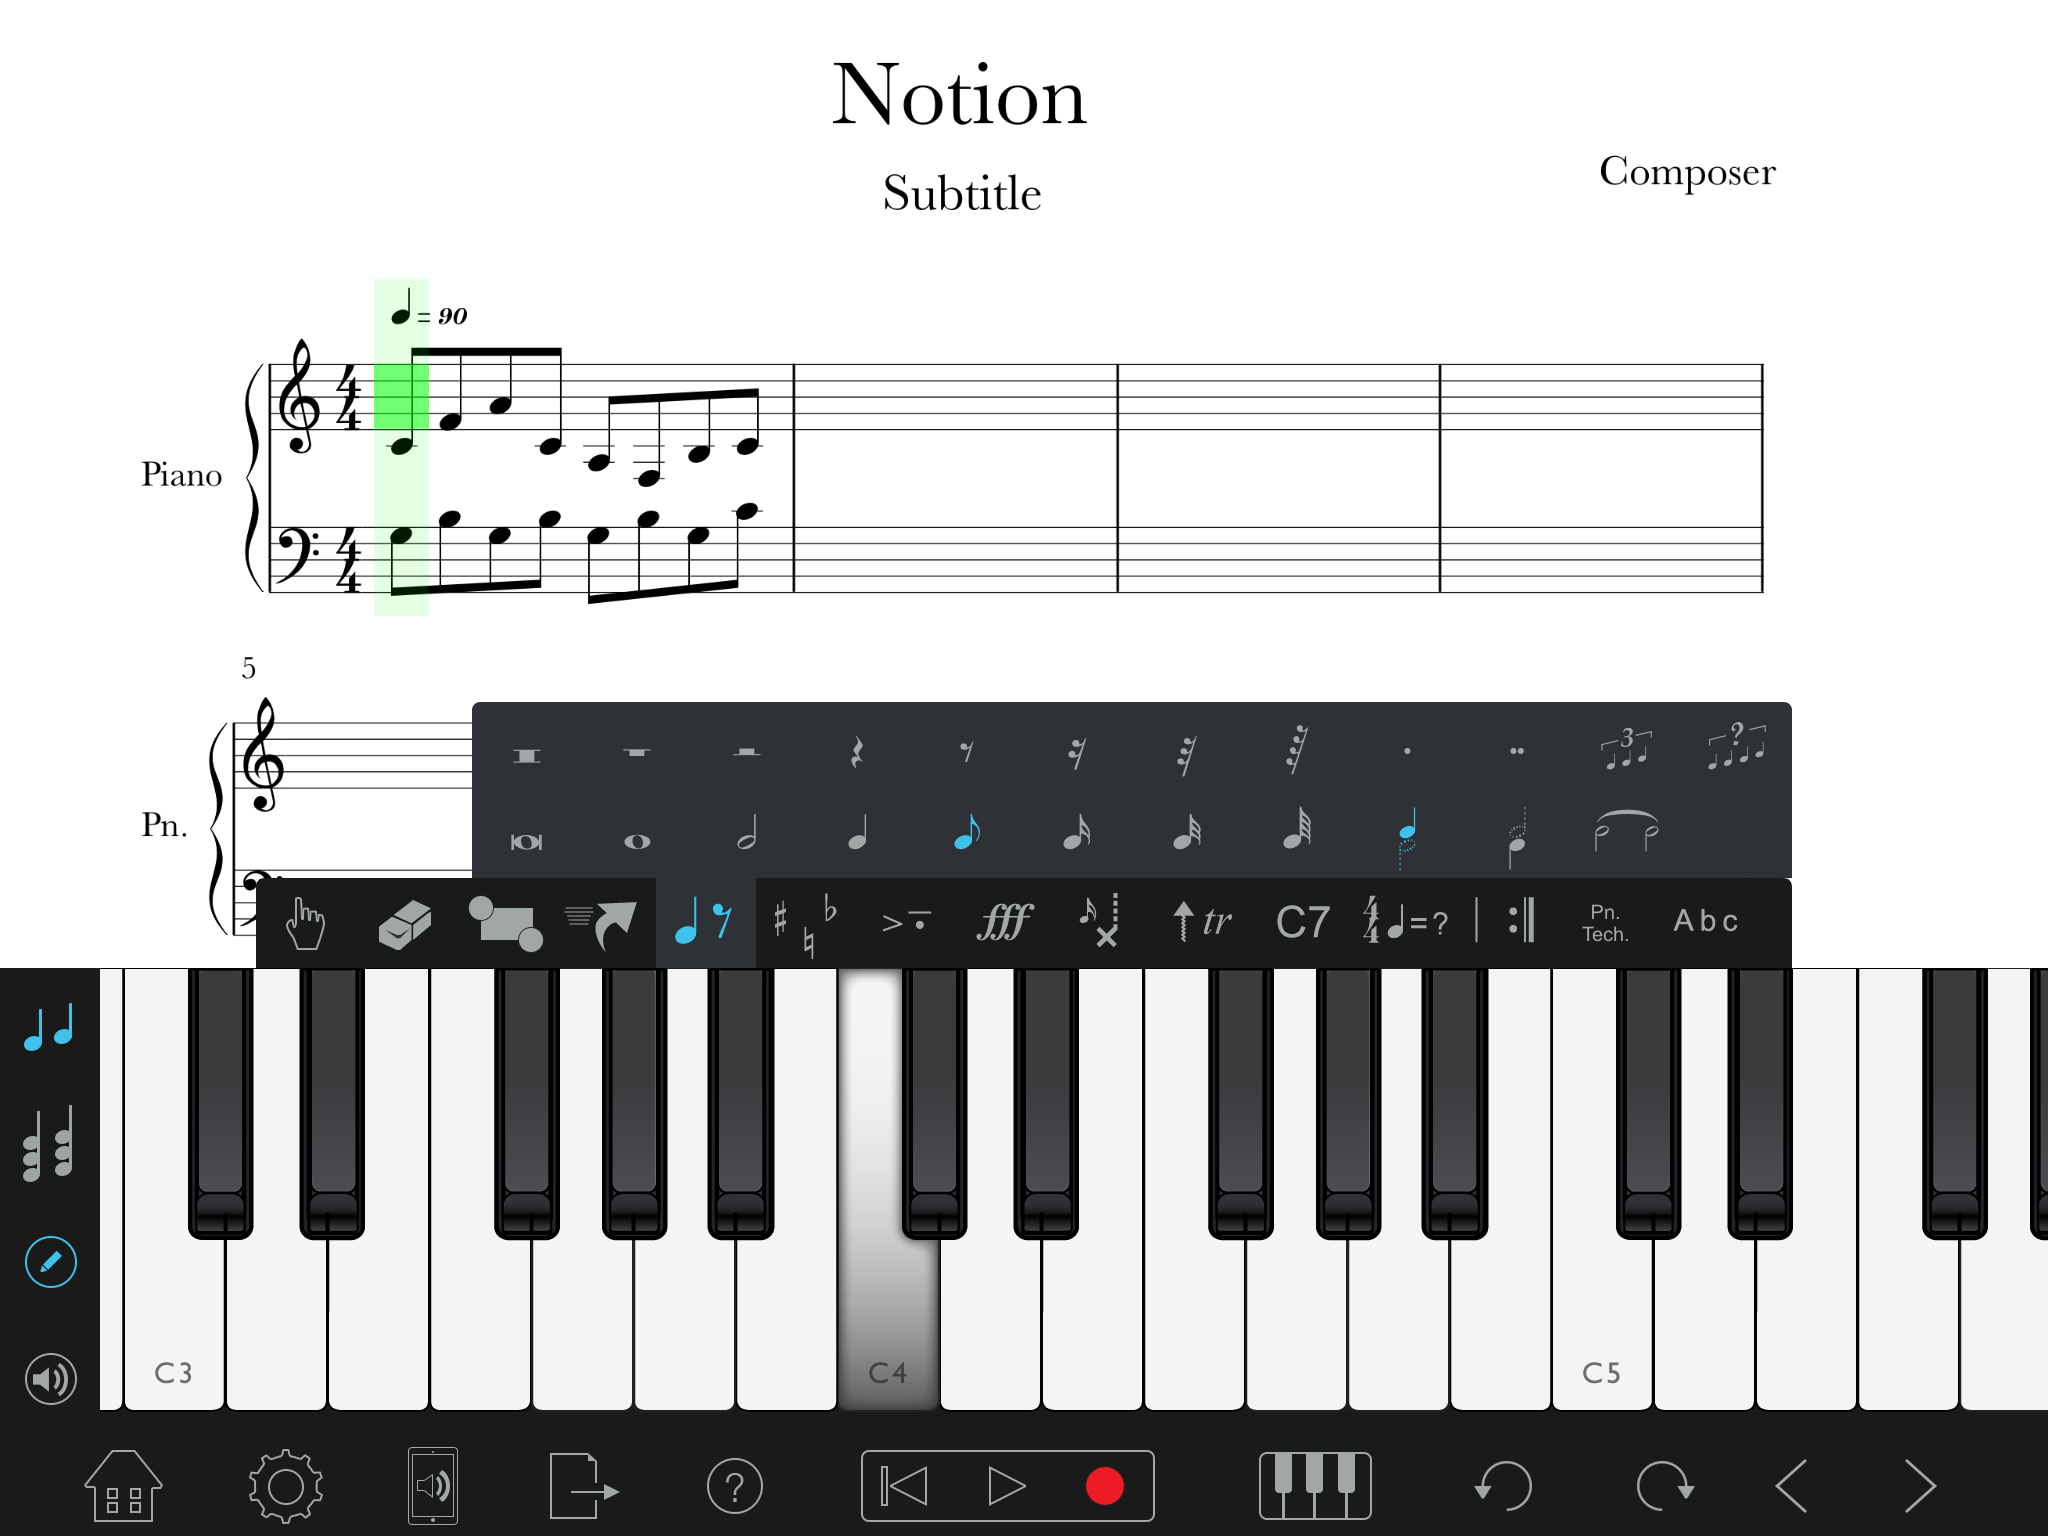
\includegraphics[scale=0.15]{figures/notion.png}}
			    \caption{The composition screen of Notion.}
			    \label{fig:notion}
			\end{figure} 

			One of Notion's most problematic features is its selection interaction. There are two (2) ways to select in Notion: the user can either hold on the measure they want to select, or press the select button in the menu. A lot of the testers were not able to figure this out initially since the hold gesture did not feel natural and the select button did not seem obvious to them. Even when they were able to figure out how to perform it, they still felt that it was tedious to perform and required too much time. This became a problem because actions like delete, cut, copy, or paste were only made available when notes or rests were selected (see Figure \ref{fig:notion_delete}). Deleting notes or rests became a hassle for the testers since they had to select first so a commonly observed workaround was that they would just use the undo feature. This did not always work well because they would sometimes want to change a note even after adding other notes. They would use undo repeatedly just to edit that note and add all the previous notes again. 

			\begin{figure}[H]
				\centering
				\frame{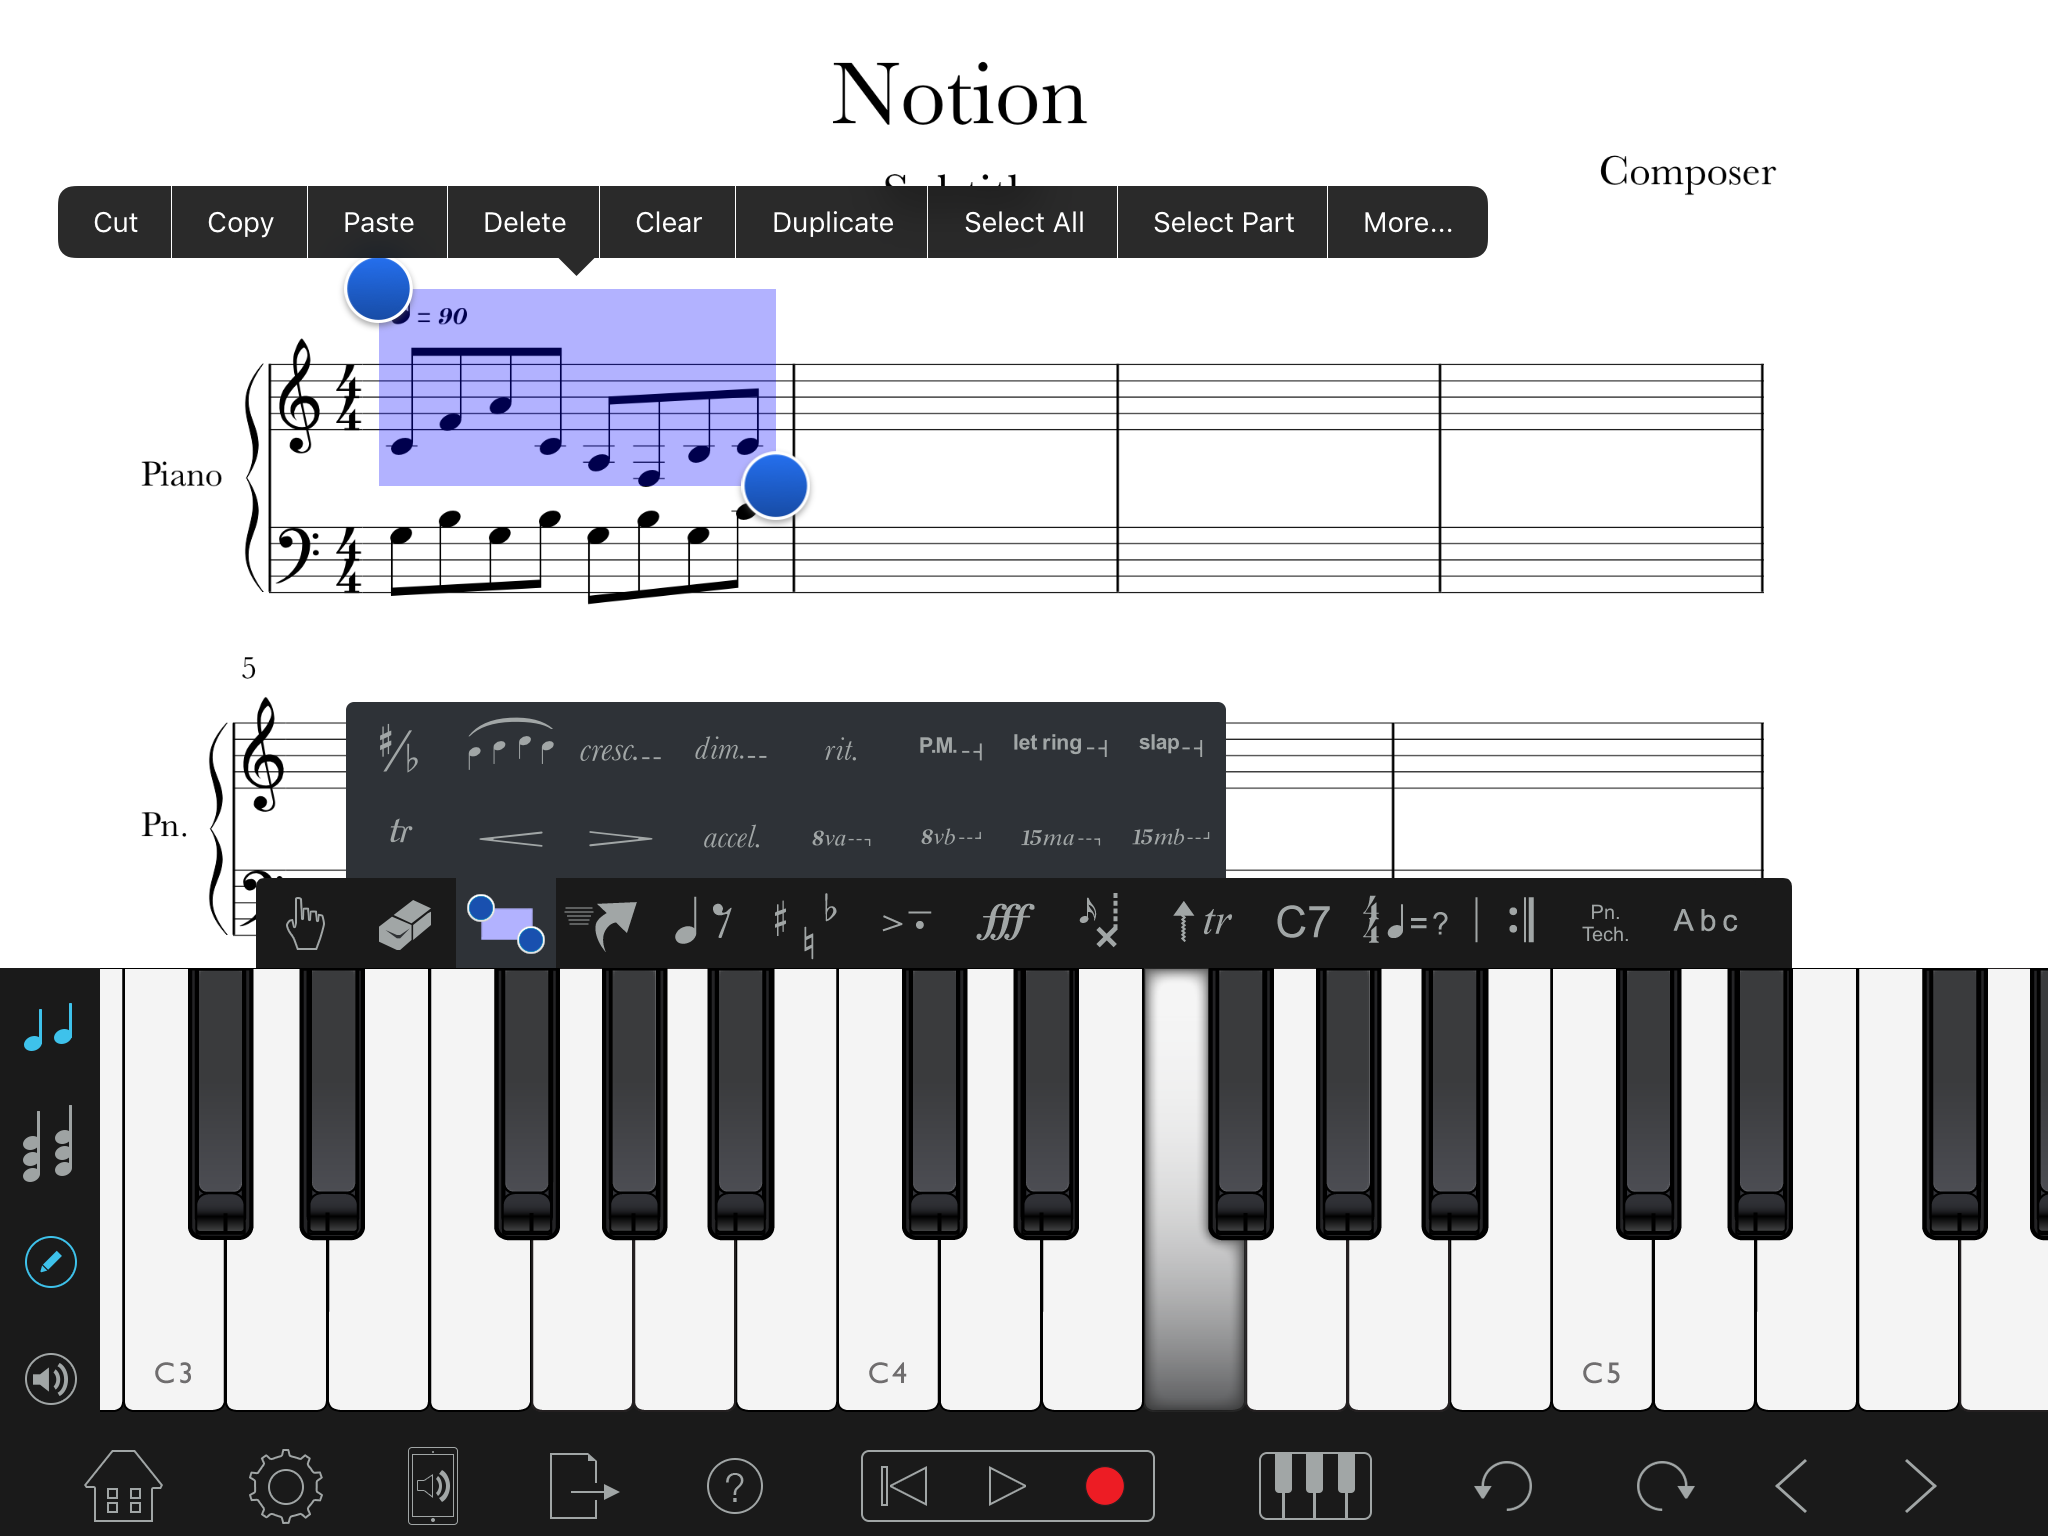
\includegraphics[scale=0.15]{figures/notion_delete.png}}
			    \caption{The composition screen of Notion with its selection menu shown.}
			    \label{fig:notion_delete}
			\end{figure} 

			\begin{comment}
			\begin{landscape}				
					\begin{longtable}{|p{3.5cm}|R{.7cm}|R{.7cm}|R{.7cm}|R{.7cm}|R{.7cm}|R{.7cm}|R{.7cm}|R{.7cm}|R{.7cm}|R{.7cm}|R{.7cm}|R{.7cm}|R{.7cm}|R{.7cm}|R{.7cm}|R{1.5cm}|}
						\caption{Notion Feature Scores per Tester for Iteration 3} \label{tab:results-notion-features-it3} \\
						  	\hline
						  	\textbf{Feature} & \textbf{T1} & \textbf{T2} & \textbf{T3} & \textbf{T4} & \textbf{T5} & \textbf{T6} & \textbf{T7} & \textbf{T8} & \textbf{T9} & \textbf{T10} & \textbf{T11}& \textbf{T12} & \textbf{T13} & \textbf{T14} & \textbf{T15} & \textbf{Average} \\ \hline

							Select or highlight notes/chords 		& 4.0 & 1.5 & 4.0 & 2.5 & 3.0 & 3.0 & 3.5 & 3.0 & 3.5 & 4.0 & 4.0 & 4.0 & 2.5 & 3.0 & 4.0 & 3.3 \\ \hline
							Add notes/chords							& 4.0 & 2.5 & 4.0 & 3.0 & 3.5 & 1.5 & 2.5 & 3.0 & 3.0 & 4.0 & 3.5 & 3.5 & 2.5 & 3.0 & 4.0 & 3.2 \\ \hline
							Edit notes/chords 							& 4.0 & 1.5 & 4.0 & 2.0 & 2.5 & 1.5 & 2.5 & 3.0 & 2.0 & 4.0 & 3.5 & 3.5 & 3.0 & 4.0 & 4.0 & 3.0 \\ \hline
							Delete notes/chords 						& 2.0 & 2.0 & 4.0 & 1.5 & 3.0 & 2.0 & 1.5 & 3.0 & 2.0 & 4.0 & 2.5 & 4.0 & 2.0 & 4.0 & 2.0 & 2.6 \\ \hline
							Cut, copy, or paste notes/chords 	& 2.5 & 1.0 & 4.0 & 1.5 & 1.0 & 3.0 & 3.5 & 3.5 & 2.5 & 4.0 & 3.5 & 4.0 & 3.0 & 2.5 & 2.5 & 2.8 \\ \hline
							Undo/redo an action 						& 4.0 & 3.5 & 4.0 & 4.0 & 3.5 & 3.5 & 4.0 & 4.0 & 4.0 & 4.0 & 4.0 & 4.0 & 4.0 & 4.0 & 4.0 & 3.9 \\ \hline
							Music Playback 								& 4.0 & 1.5 & 4.0 & 3.0 & 3.0 & 2.5 & 3.5 & 3.0 & 2.5 & 2.0 & 4.0 & 4.0 & 4.0 & 3.5 & 4.0 & 3.2 \\ \hline

							\multicolumn{16}{|l|}{\textbf{Average}} & 3.1 \\ \hline

					\end{longtable}
				\end{landscape}

				\begin{landscape}				
					\begin{longtable}{|p{3.5cm}|R{.7cm}|R{.7cm}|R{.7cm}|R{.7cm}|R{.7cm}|R{.7cm}|R{.7cm}|R{.7cm}|R{.7cm}|R{.7cm}|R{.7cm}|R{1.5cm}|}
						\caption{Notion Feature Scores per Tester for Iteration 4} \label{tab:results-notion-features-it4} \\
						  	\hline
						  	\textbf{Feature} & \textbf{T1} & \textbf{T2} & \textbf{T3} & \textbf{T4} & \textbf{T5} & \textbf{T6} & \textbf{T7} & \textbf{T8} & \textbf{T9} & \textbf{T10} & \textbf{T11} & \textbf{Average} \\ \hline

						  	Select or highlight notes/chords 		& 2.0 & 3.0 & 3.3 & 3.3 & 2.7 & 4.0 & 2.0 & 2.7 & 4.0 & 4.0 & 3.3 & 3.1 \\ \hline
							Add notes/chords 							& 2.3 & 3.0 & 3.7 & 3.7 & 3.0 & 3.7 & 1.7 & 2.0 & 4.0 & 4.0 & 4.0 & 3.2 \\ \hline
							Edit notes/chords 							& 2.0 & 3.0 & 4.0 & 3.0 & 2.0 & 4.0 & 1.7 & 1.7 & 4.0 & 4.0 & 1.7 & 2.8 \\ \hline
							Delete notes/chords 						& 1.7 & 3.7 & 2.0 & 4.0 & 2.7 & 4.0 & 2.7 & 2.7 & 4.0 & 2.7 & 4.0 & 3.1 \\ \hline
							Cut, copy, or paste notes/chords 	& 1.7 & 2.0 & 3.0 & 3.7 & 3.0 & 4.0 & 2.3 & 3.7 & 4.0 & 4.0 & 3.3 & 3.2 \\ \hline
							Undo/redo an action 						& 4.0 & 3.7 & 4.0 & 4.0 & 4.0 & 4.0 & 2.3 & 3.0 & 4.0 & 3.0 & 4.0 & 3.6 \\ \hline
							Music Playback 								& 3.0 & 4.0 & 4.0 & 4.0 & 4.0 & 4.0 & 3.0 & 2.0 & 4.0 & 3.7 & 2.0 & 3.4 \\ \hline

							\multicolumn{12}{|l|}{\textbf{Average}} & 3.2 \\ \hline

					\end{longtable}
				\end{landscape} 

				\end{comment}
	
	% section comparative_analysis (end)


